\documentclass{article}

% if you need to pass options to natbib, use, e.g.:
% \PassOptionsToPackage{numbers, compress}{natbib}
% before loading nips_2016
%
% to avoid loading the natbib package, add option nonatbib:
% \usepackage[nonatbib]{nips_2016}

\usepackage[final]{nips_2016}

% to compile a camera-ready version, add the [final] option, e.g.:
\usepackage{nips_2016}

\usepackage[utf8]{inputenc} % allow utf-8 input
\usepackage[T1]{fontenc}    % use 8-bit T1 fonts
\usepackage{hyperref}       % hyperlinks
\usepackage{url}            % simple URL typesetting
\usepackage{booktabs}       % professional-quality tables
\usepackage{amsfonts}       % blackboard math symbols
\usepackage{nicefrac}       % compact symbols for 1/2, etc.
\usepackage{microtype}      % microtypography
\usepackage{graphicx}
\usepackage{subfig}
\usepackage{amsmath}
\usepackage{relsize}
\usepackage{algorithm}
\usepackage[noend]{algpseudocode}

\newcommand\tab[1][1cm]{\hspace*{#1}}

\renewcommand{\vec}[1]{\mathbf{#1}}

\title{A Neural Architecture for Unsupervised Temporal Pattern Recognition}

\author{
  Shady El Damaty \\
  Department of Neuroscience\\
  Georgetown University\\
  Washington, D.C. 20067 \\
  \texttt{se394@georgetown.edu} \\
  %% examples of more authors
  \And
  James Maguire \\
  Department of Linguistics \\
  Georgetown University \\
  Washington, D.C. 20067\\
  \texttt{jrm346@georgetown.edu} \\
}
% ***********************************************
%% 			  	  BEGIN DOCUMENT
% ***********************************************
\begin{document}
\maketitle
% ***********************************************
%% 					ABSTRACT
% ***********************************************
\begin{abstract}
In this paper we present a novel neuron architecture for unsupervised time dependent neural networks. We provide a new delay function, based on a mixture of Beta distributions, which addresses some of the problems with previous work in this area. In addition we also present a new method of thresholding the potential of a neuron based on input activations from both before and after the neuron spikes. Preliminary results over two simple patterns show extremely high performance on an unsupervised pattern segmentation task, learning in both clean and noisy environments.   
\end{abstract}
% ***********************************************
%%				  INTRODUCTION
% ***********************************************
\section*{Introduction}
Noisy time series signals pose numerous challenges for pattern recognition algorithms.  The absence of delimiters to signify the beginning and end of a pattern require either prior knowledge of the pattern's properties or a capability for identifying a pattern based on it's statistical properties within the input stream. Neural networks have shown great promise for temporal pattern recognition.  A popular approach for detecting unique patterns embedded in a noisy signal have centered around representing the relative inputs of the constituent features that compose a pattern as a system of time delays relative to pattern onset (Hopfield 1996, Tank \& Hopfield 1987). Supervised algorithms with time-delay neural networks have previously shown high performance rates ($>98\%$) for classification of consonant phonemes (Waibel et al. 1989). The hidden layers within this model had learned to represent acoustic-phonetic features for classification of phonemes nested  within a noisy signal.  Current research has focused on developing unsupervised methods to learning acoustic-phonetic features in real time.  Spike-Timing Dependent Plasticity (STDP) is an unsupervised learning rule derived from neurophysiological experiments (Izhikevich 2006).  Neurons with an STDP learning rule potentiate their weights as a function of the relative time between input arrival and the neuron's firing time.  Inputs that arrive before the neuron emits a spike are potentiated whereas those that arrive afterwards are depotentiated. A STDP learning rule drives the neuron to fire only for those inputs that actually contributed to its activity. Recent work has implemented STDP with time-delay learning for semi-unsupervised learning of weighted delays for spatio-temporal pattern recognition (Moisy et al. 2015).  Others have implemented unsupervised STDP with time-delay learning by initializing a random system of time delays and retaining only those delays that represent the temporal structure of the input (Rekabdar 2015). In this paper, we build upon previous literature for fully-unsupervised learning of time-delays using a novel delay function based on the beta distribution.

% ***********************************************
%% 			  PATTERN REPRESENTATION
% ***********************************************
\section*{Pattern Representation}
Consider a noisy signal $g(\vec{f}, \vec{t})$ with spatial features $\vec{f}=[f_1 ... f_i]$ defined over a time interval $\vec{t}=[t_1 ... t_k]$. A unique first-order pattern within $g(\vec{f}, \vec{t})$ is defined as 
% ***********************************************
% -- definition of pattern
\begin{align}
\xi = \big( (f_{m},t_{o}) ... (f_{n},t_e) \big) \tab n \geq m > 0
\label{eq:pattern}
\end{align}
% ***********************************************
where $\xi$ is a list of elements chosen from $\vec{f}$ and appearing within $g(\vec{f},\vec{t})$ between each pattern start, $t_0$, and end, $t_e$, for a pattern duration $c=t_e-t_o$. Each characteristic feature, $f_x$, on the interval $x \in [m ... n]$ may appear more than once in $\xi$ and is thus associated with a vector of times, 
% ***********************************************
% -- definition of characteristic feature times
\begin{align}
\boldsymbol{\tau}_{f_x}=[\tau_p ... \tau_j]
\end{align}
% ***********************************************
where $j$ is the total number of times $f_x$ is present within $c$. The spatio-temporal signature of $\xi$ is the collected set of all orderings in time of every characteristic feature composing $\xi$,
\begin{align}
\boldsymbol{T}_\xi=[\boldsymbol{\tau}_{f_{m}} ... \boldsymbol{\tau}_{f_{n}}]
\end{align}
The consistent appearance of $\xi$ at times $\boldsymbol{T}_\xi$ constitutes a statistically reproducible pattern that may be learned by an unsupervised algorithm sensitive to the statistical properties of $g(\vec{f},\vec{t})$. Pattern $\xi$ is called a first-order pattern in time series $g(\vec{f},\vec{t})$ if the signature $\vec{T}_\xi$ is a statistically regular sequence unique to $\xi$ and not any other overlapping patterns in $g(\vec{f},\vec{t})$.
%%What do you mean by statistically regular?
%%These points here are really interesting regarding how a pattern may be defined as a statistically regular sequence of activation times of a given feature vector set.
%%At some point, it may be worthwhile to explore the idea that a sequence becomes a pattern when the conditional probabilities of the elements in the sequence approaches some critical p value.
%%There may also be useful forays in information theory regarding the minimum message length required to transmit a signal across a noisy channel.  The length of a pattern is maximized when the features all occur at an equal probability.  However, once redundancy starts being introduced by generating patterns that always co-occur together then the length is minimized.
%%Also note that the N-gram conditional entropy of a sequence of features that compose a pattern greatly increases at the transition between patterns.
% ***********************************************
%% 			  	 Architecture
% ***********************************************
\section*{Neuron Architecture} The set of features that characterize a given $\xi$ nested within a noisy time series may be detected by a neuron, $n$, receiving feedforward input from a set of feature detector units, $\vec{s}=[s_1 ... s_i]$, in one-to-one correspondence with $\vec{f}$.  

Each unit in $\vec{s}$ converts a binary value indicating the presence of an input at a time $\tau_{s} \in \vec{T_S}$ into a time-varying signal driving $n$ over interval $\vec{t}$. Recognition of $\xi$ occurs when the activity of $n$ exceeds a suprathreshold value, $\gamma$, and emits a spike to signal the detection of the spatio-temporal signature, $\vec{T_{S}}$ . The threshold must be set sufficiently high enough to filter out spurious activation and also such that $n$ will only fire when all inputs arrive at the same time. Coincident arrival may only occur if all inputs activate at the same time or if the arrival time of the input from each unit in $\vec{s}$ is sufficiently delayed relative to the final detected feature. This constraint is satisfied if each input has a delay function $\vec{d}=[d_{s_1}(z) ... d_{s_i}(z)]$, where $z$ is a positive real value and the neuron potential is written as the summation over the input activations within a window since the neuron last fired, $\phi$, 
%***********************************************
%			Definition of Potential
\begin{align}
h(t, \phi) = \mathlarger{\sum_{\boldsymbol{\tau_s} \in \phi}}d_s(t-\vec{\tau_s}) \tab
\end{align}
%***********************************************
such that $t$ is the current time of the signal $g(\vec{f},\vec{t})$.  This architecture is illustrated in Figure \ref{fig:1A}. The neuron fires a binary spike at time $\tau_{n}$ if $h(t, \phi) > \gamma$. However, if the temporal structure of activated inputs does not correspond to $\vec{T}_\xi$ then the arrival times are all out of phase with each other and the potential of the neuron never exceeds $\gamma$ as shown in Figure \ref{fig:1B}. 
% ***********************************************
%% 			  	 % Figure 1
% ***********************************************
\begin{figure}[ht]   
\centering
\subfloat{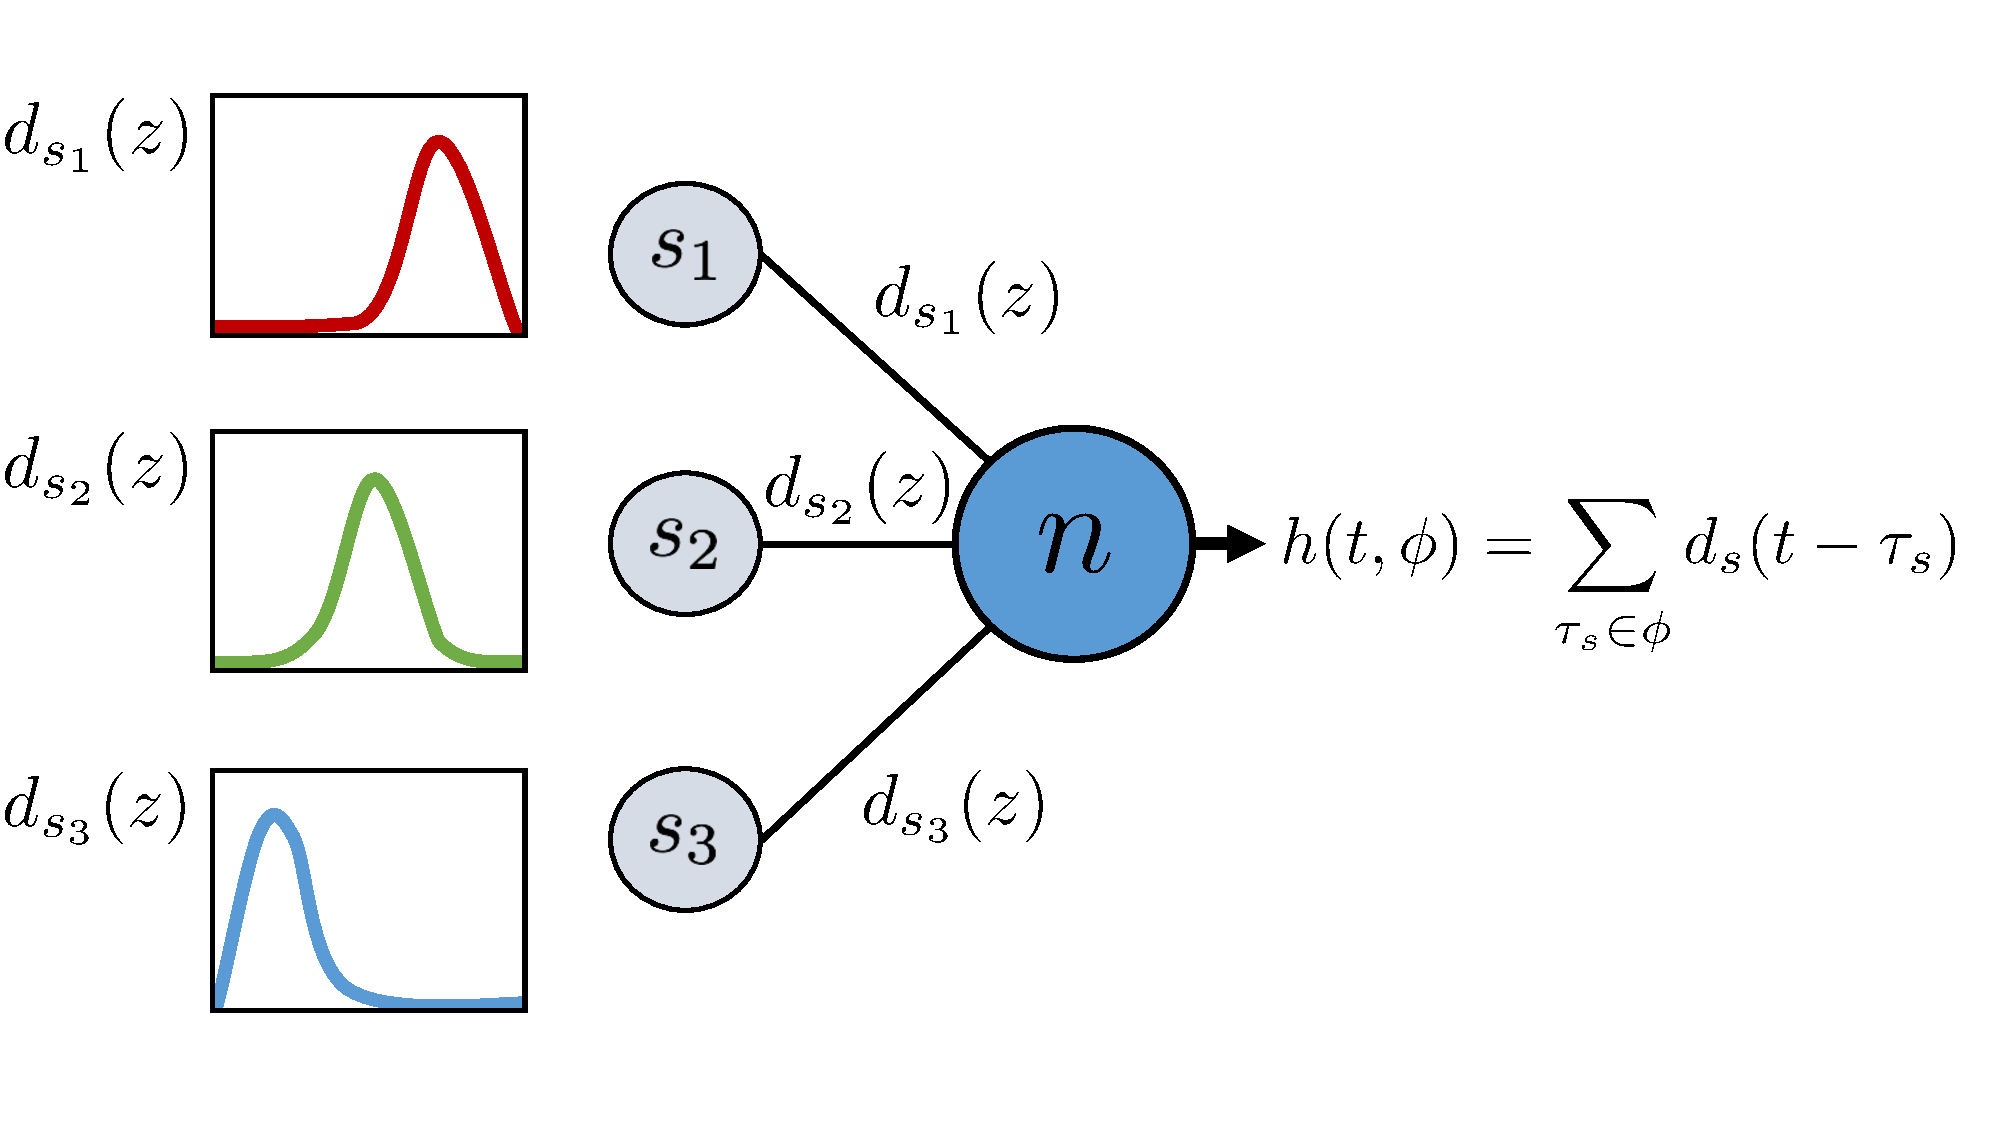
\includegraphics[width=0.5\textwidth, keepaspectratio]{Fig1A.pdf}\label{fig:1A}}
\subfloat{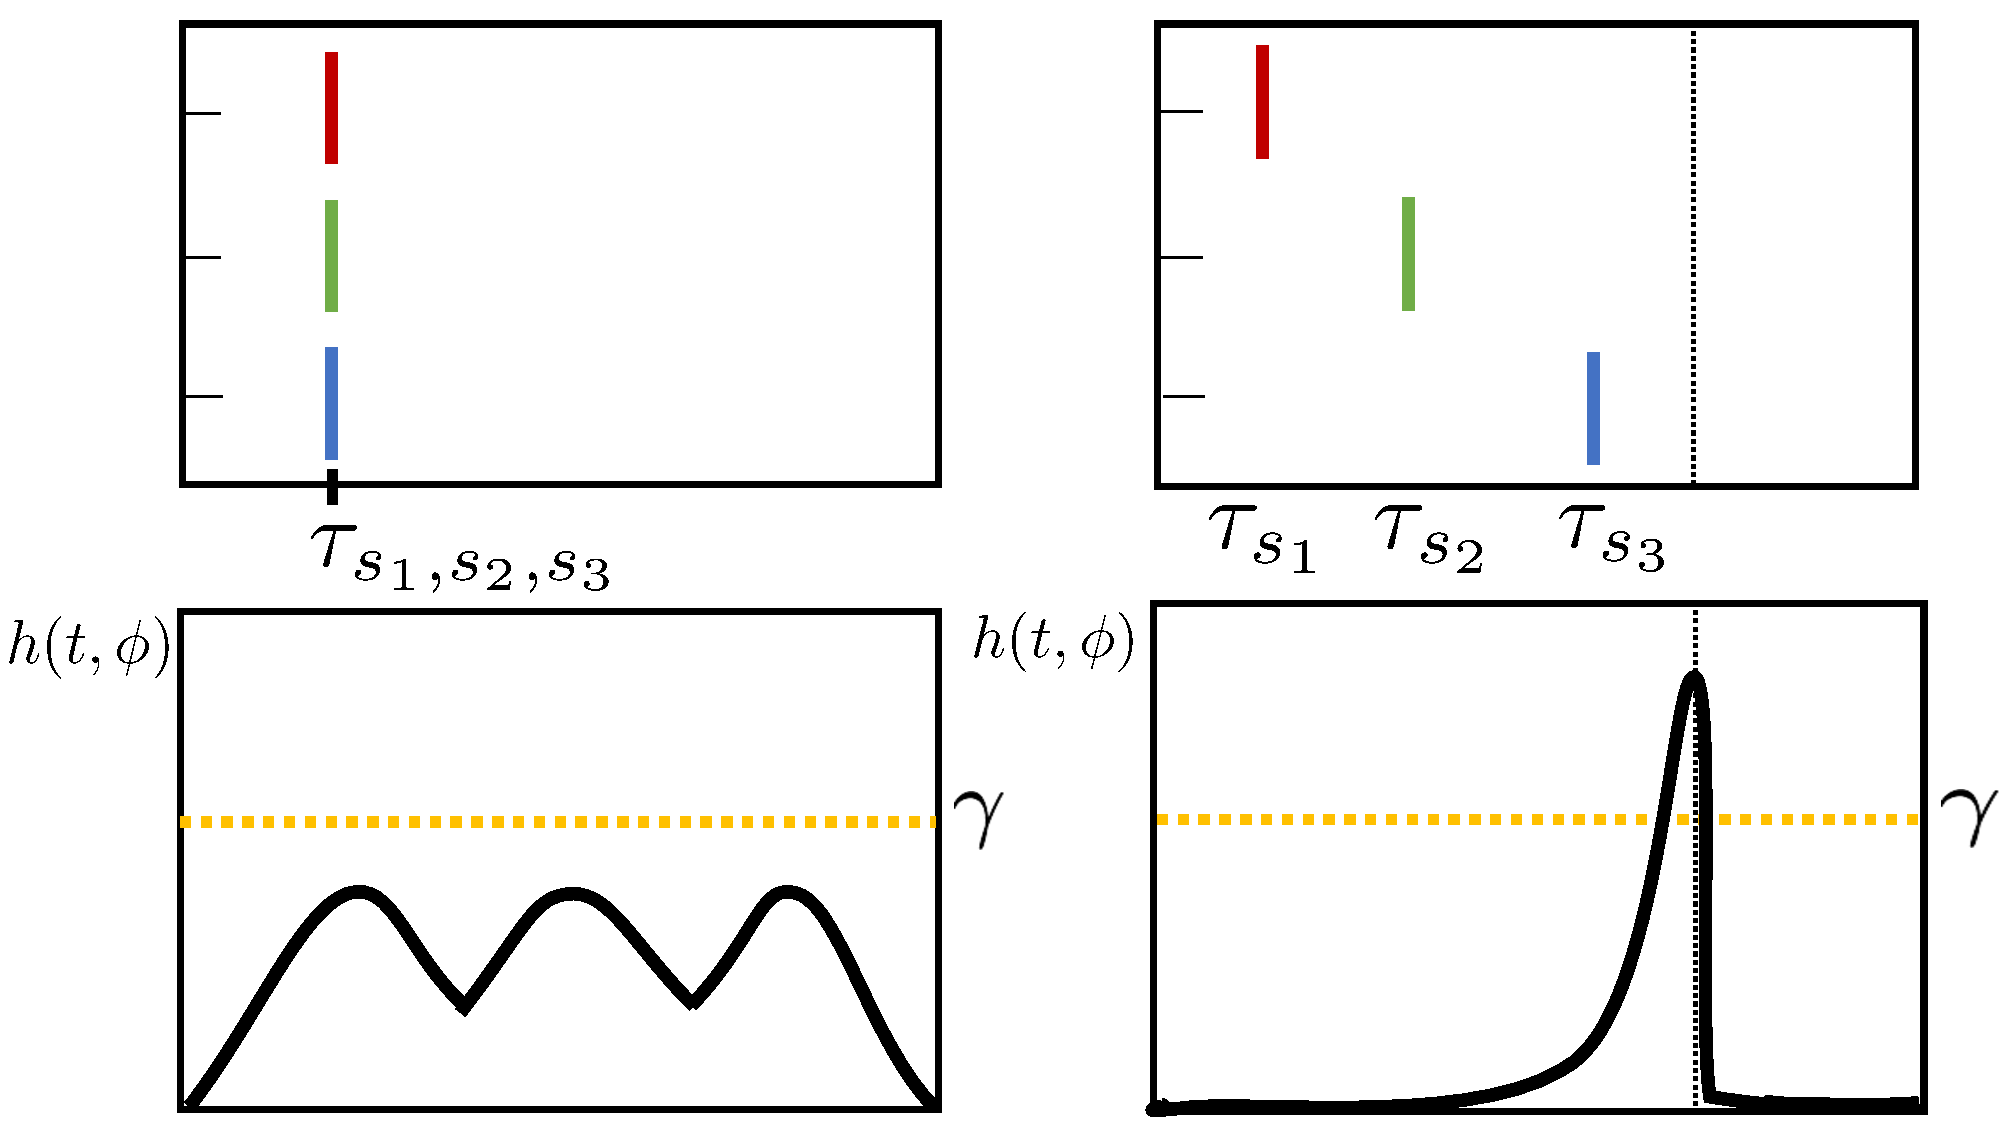
\includegraphics[width=0.5\textwidth, keepaspectratio]{Fig1B.pdf}\label{fig:1B}}
\caption[]{\textbf{Architecture of a Single Pattern Detecting Neuron}}
\end{figure}      
% ***********************************************
%% 			  	 Delay Function
% ***********************************************
\subsection*{Novel Delay Function}
% ***********************************************
%% 			  	 % Figure 2
% *********************************************** 
The choice of the delay function is crucial for achieving the previously mentioned constraints for $n$ emitting a spike in response to a detected pattern $\xi$. A popular choice in the literature is the application of weighted fixed delay functions, where the value of the function is dependent solely on the time since input activation, $d_{fixed}(z)$.  An example of a  weighted fixed delay function appears in Figure \ref{fig:2}.  Learning with this kind of delay function consists of modulating the height of the delay function, $d_{fixed}(z)$, to push the pattern-detecting neuron over threshold.  A major limitation of these models is that such a representation does not allow for the peak value of the delay function to be shifted in time according to the 
temporal statistics of the pattern to be learned.        
\begin{figure}[ht]   
\centering
\subfloat{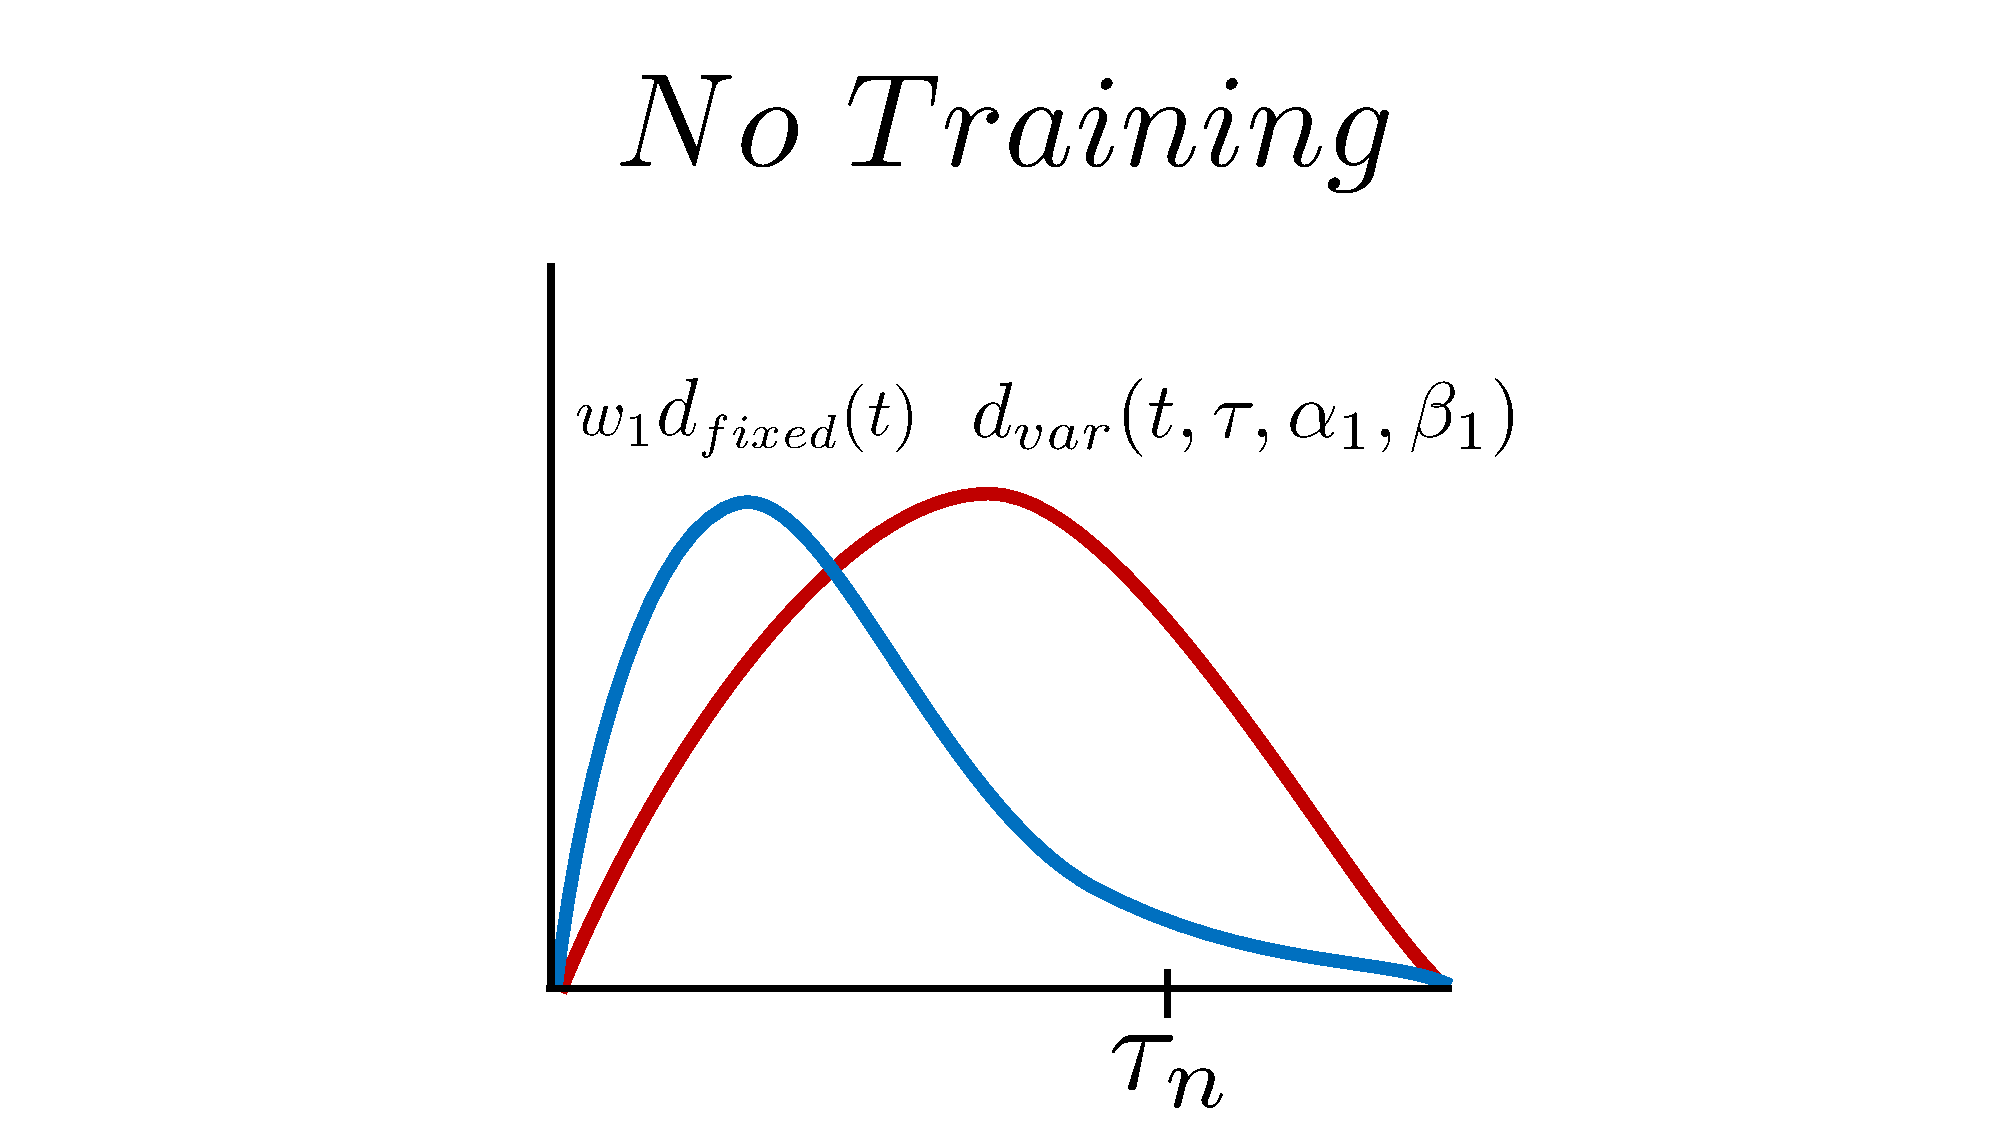
\includegraphics[width=0.25\textwidth,height=3.5cm]{Fig2A.pdf}}
\subfloat{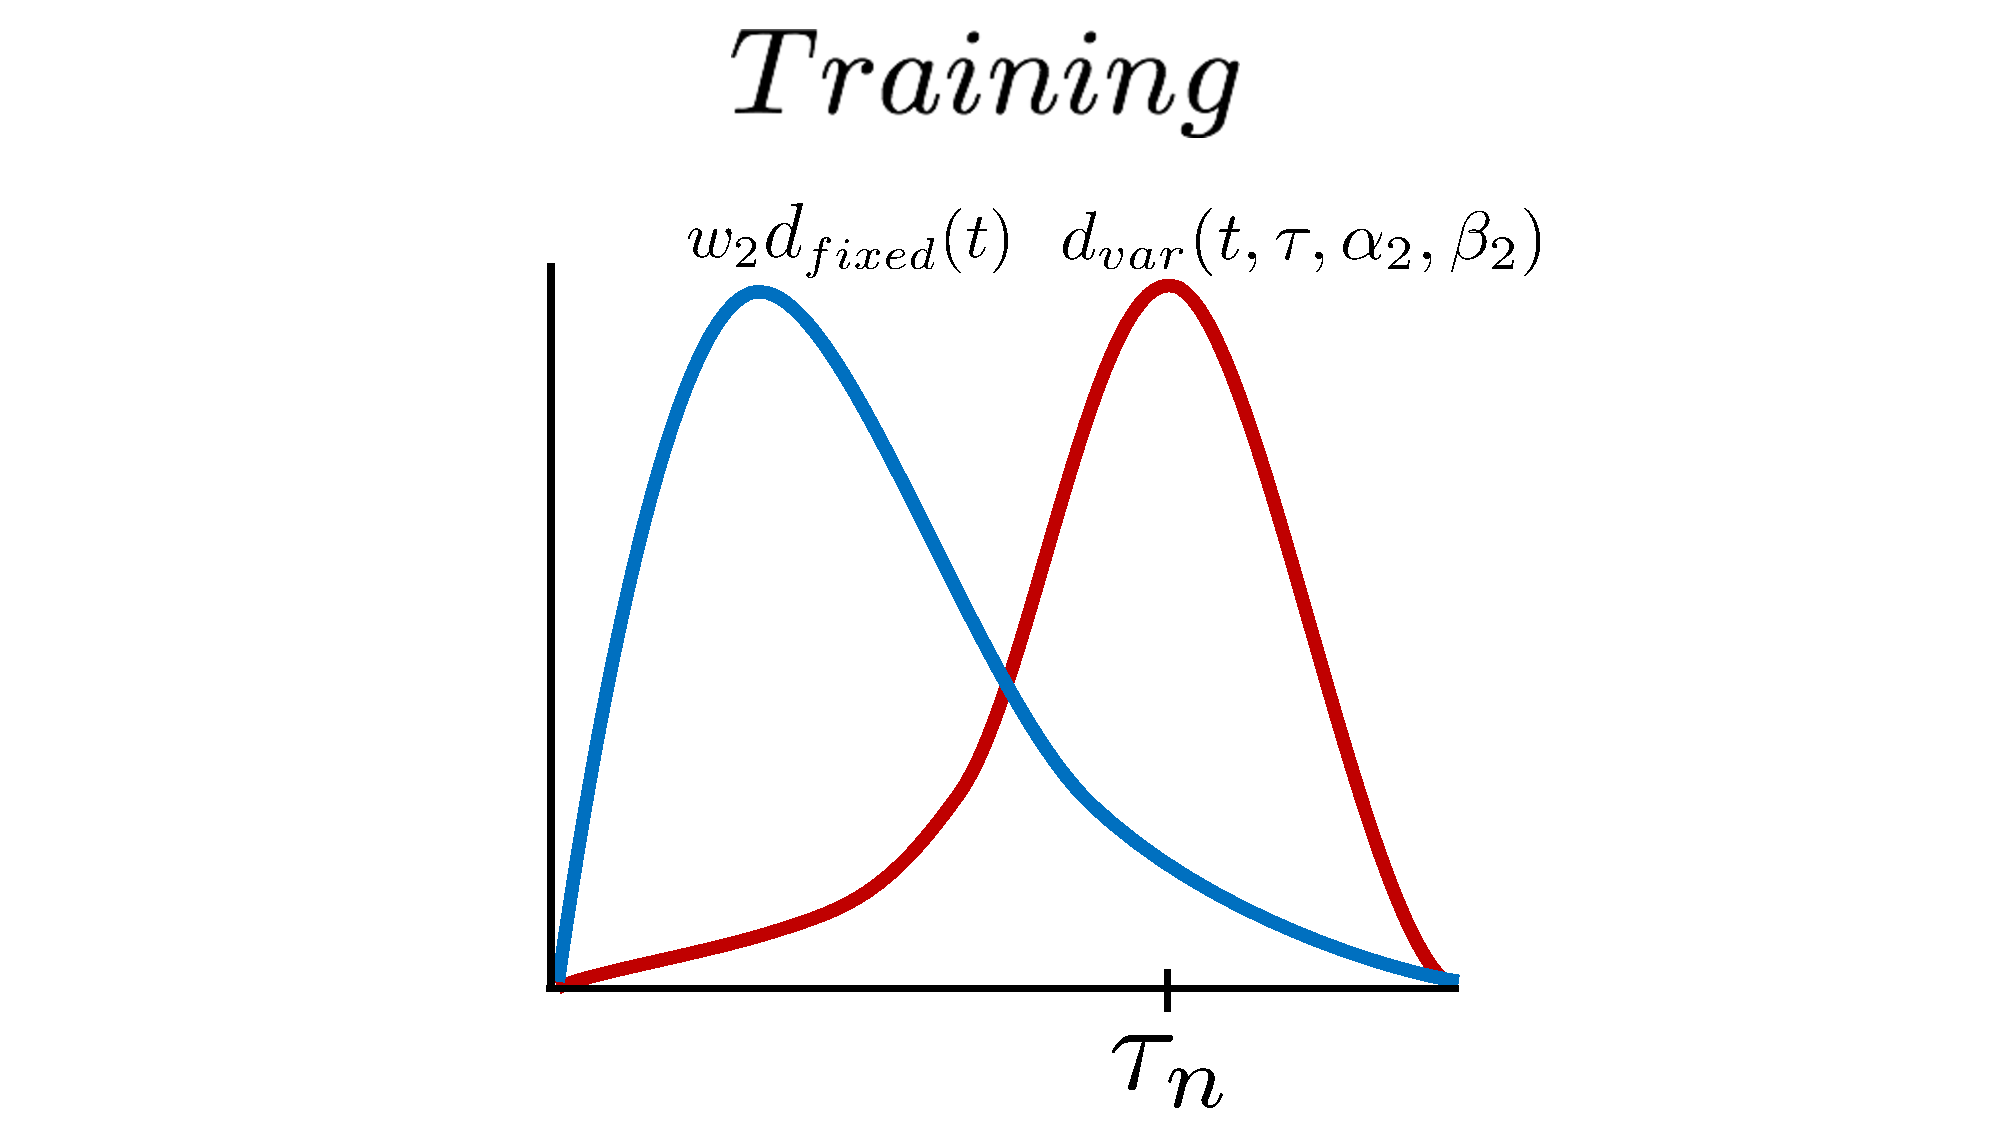
\includegraphics[width=0.25\textwidth,height=3.5cm]{Fig2B.pdf}}
\caption{\textbf{Fixed vs. Variable Delay Functions}}
\label{fig:2}
\end{figure} 
The beta distribution is ideal for representing temporal delays due to its adjustable hyperparameters, $\alpha, \beta$.  These hyperparameters can be adjusted to move the peak value of the distribution in any direction (Figure \ref{fig:2}).  This means that the peak values of the input functions can be adjusted to arrive coincidentally thus creating a spike in the potential of the neuron as observed in Figure \ref{fig:1B}.  Taking inspiration from spike-timing dependent plasticity (STDP) models, the peak of the delay function is skewed based on the relative difference between input activation,  $\tau_s$, and neural firing time, $\tau_n$.  Thus the arrival time of the peak of the delay function is learned to ensure coincidental arrival across inputs at firing time. The beta distribution can be defined as function of the gamma distribution, $\Gamma$, where $z \in [0,1]$ and $\alpha,\beta \geq 0$
\begin{align}
\beta(z,\alpha,\beta) = \frac{\Gamma(\alpha+\beta)}{\Gamma(\alpha)\Gamma(\beta)} \cdot{} z^{\alpha-1}(1-z)^{\beta-1}
\label{eqn:gamma}
\end{align}
The maximal duration of the delay function is a hyperparameter, $c$, which should be selected based on the expected length of the input pattern.  The pattern duration must be appropriately scaled since the beta distribution is only defined on the interval $z \in [0,1]$. In order to calculate the value of the beta delay function at time $t$ with an input activation time $\tau_{s_i}$, $z$ is defined as:
\begin{align}
z=\frac{ (t- \tau_{s_i}) }{c}
\label{eqn:x}
\end{align}
The variable delay function $d_{var}$ with hyperparameters $\alpha$ and $\beta$ updated during learning, can be written as:
\begin{align}
d_{var}(t,\tau,\alpha,\beta) =  \frac{\Gamma(\alpha+\beta)}{\Gamma(\alpha)\Gamma(\beta)} \cdot{} \bigg(\frac{ t- \tau_{s_i} }{c}\bigg)^{\alpha-1}\bigg(1-\frac{ t- \tau_{s_i} }{c}\bigg)^{\beta-1}
\label{eqn:delay}
\end{align}
% ***********************************************
%% 			  	 	Mixtures
% ***********************************************
\subsection*{Beta Mixtures}
% ***********************************************
%% 			  	 	%FIGURE 3
% ***********************************************       
While the definition of $d_{var}$ with only a single beta distribution allows for learning the delay time of an input which is activated only once within the pattern window, $c$, it fails to approximate the appropriate delay for when an input activates multiple times within $c$. In order to resolve this problem, $d_{var}$ is defined as a mixture of beta distributions as follows, 
\begin{align}
d_{var}(t,\tau,\boldsymbol{\alpha},\boldsymbol{\beta}) = \mathlarger{\mathlarger{\sum}}_{\alpha,\beta \ \in \ \boldsymbol{\alpha},\boldsymbol{\beta}} \frac{\Gamma(\alpha+\beta)}{\Gamma(\alpha)\Gamma(\beta)} \cdot{} \bigg(\frac{ t- \tau_{s_i} }{c}\bigg)^{\alpha-1}\bigg(1-\frac{ t- \tau_{s_i} }{c}\bigg)^{\beta-1}
\label{delay}
\end{align}
where $\boldsymbol{\alpha}$ and $\boldsymbol{\beta}$ are vectors of $\alpha$ and $\beta$ values respectively. If $f_{var}$ is activated in the correct sequence, the multiple peaks corresponding to different input activation times will all arrive in phase. Coincident input will drive the neuron potential, now defined as:
\begin{align}
h(t,\phi) = \mathlarger{\sum_{\tau_s \ \in \ \phi}} d_{var}(t,\tau,\boldsymbol{\alpha},\boldsymbol{\beta})
\end{align}
to spike and exceed $\gamma$.  The difference between a mixture and a single component distribution is exemplified in figure \ref{fig:3}.
\begin{figure}[ht]   
\centering
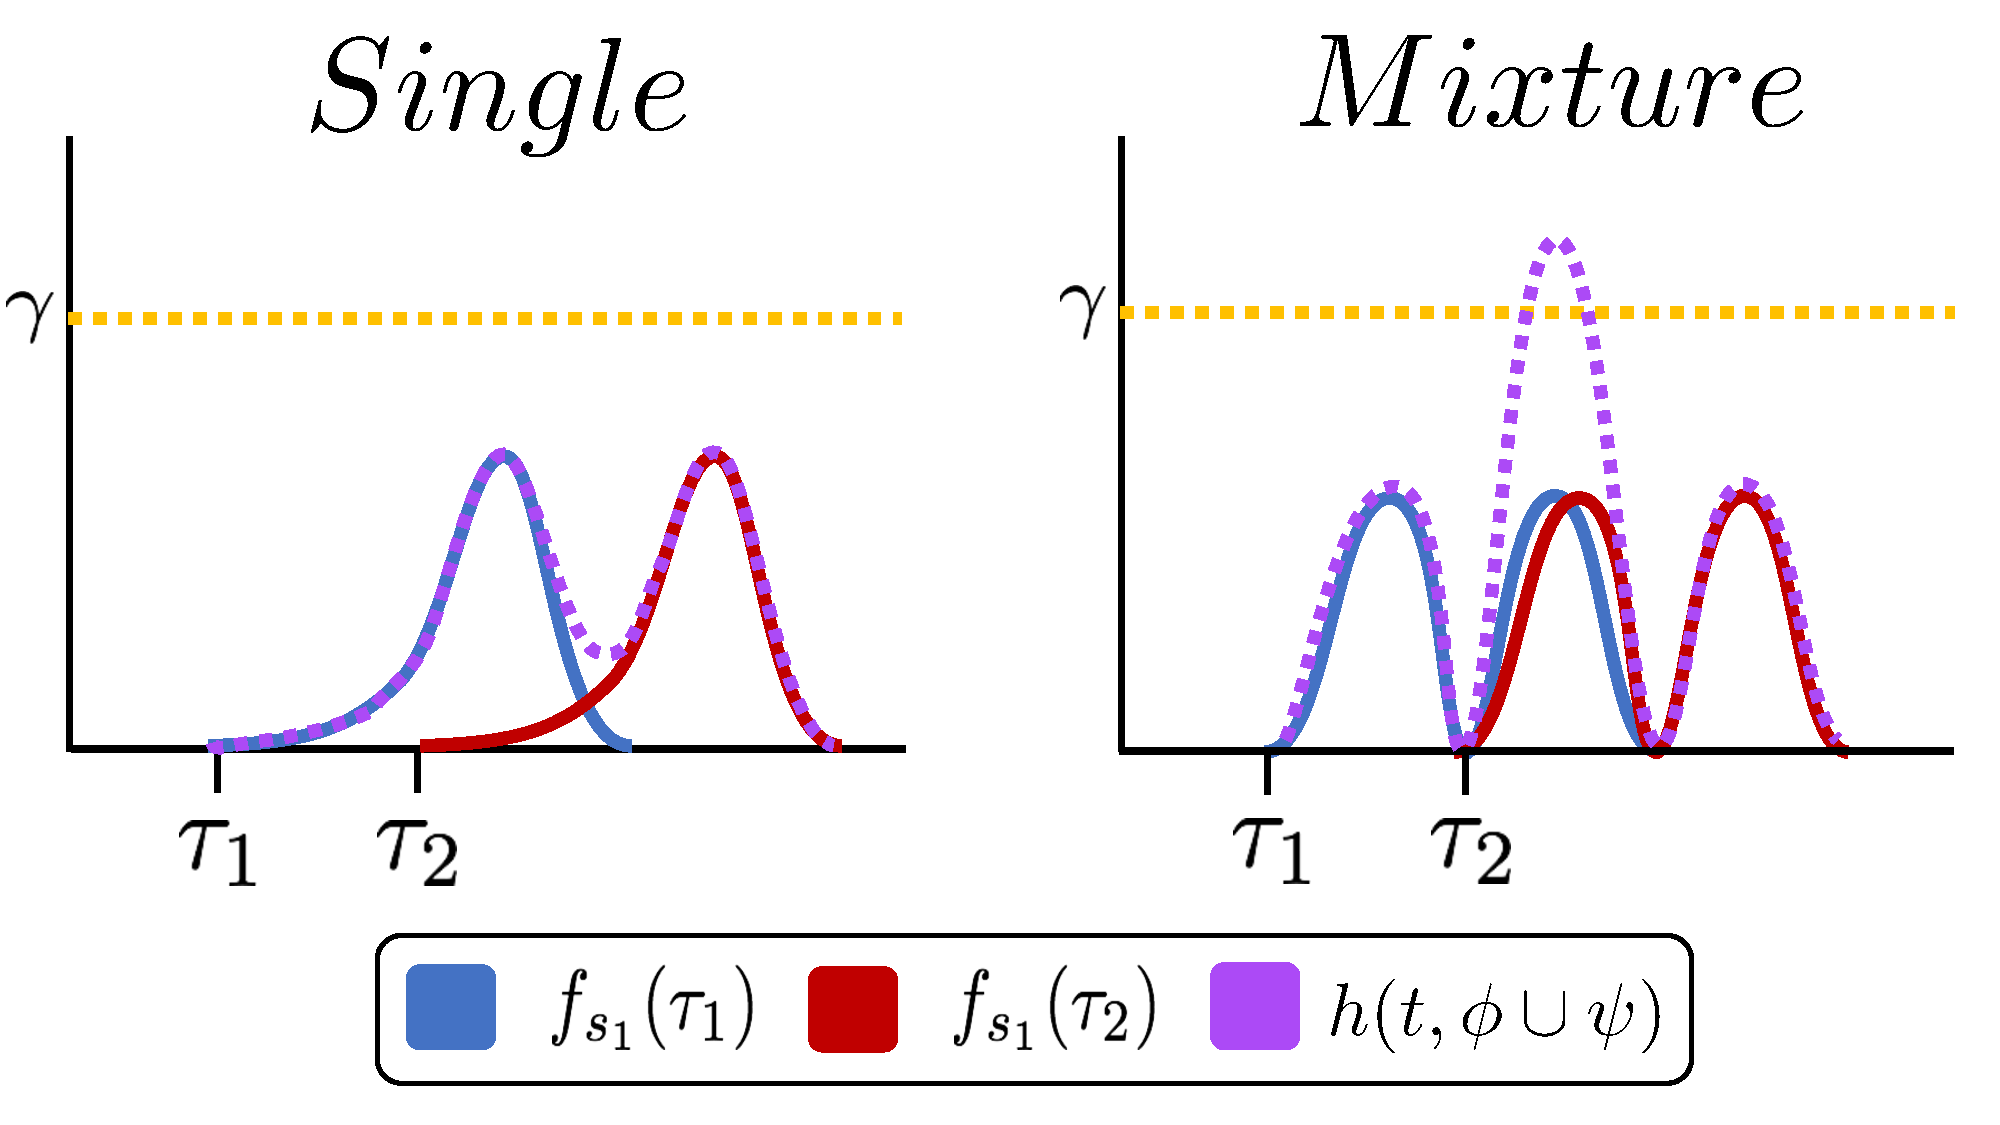
\includegraphics[width=0.5\textwidth]{Fig3}
\caption{\textbf{Representing Multiple Inputs with a Beta Mixture}}
\label{fig:3}
\end{figure} 
% ***********************************************
%% 			  	Thresholding
% ***********************************************
\subsection*{Setting the Threshold} 
Integrate and fire neurons generally possess either a fixed or variable threshold which is dependent on the potential of the neuron at firing.  The problem with a fixed threshold is that a static $\gamma$ causes the firing time, $\tau_n$ of the neuron to be prior to the end of the pattern, generally causing $\tau_n$ to move to the beginning of the pattern. This is problematic as the neuron only detects the onset and not the complete duration of the pattern.  Some groups have addressed this by assembling multiple neurons to represent a single pattern. A static threshold can also be easily overwhelmed by increased noise in the signal. This issue can be addressed with a single neuron that fires at the end of $\xi$ by  defining,
\begin{align}
\phi = \{ \tau \ | \ (t-\tau_s) \leq c  \ \ \ and  \ \ \ \tau_n < \tau_s\} \\
\psi = \{ \tau \ | \ (t-\tau_s) \leq c  \ \ \ and  \ \ \ \tau_n \geq \tau_s\}
\end{align}
where $\phi$ is the set of input activations within the window, $(t-\tau_s) \leq c$, since the neuron last fired, $\tau_n < \tau_s$, and $\psi$ is the set of activations within the window prior to the neuron's last firing $\tau_n \geq \tau_s$. In contrast to previous work, where the thresholds are dependent on the potential of the network at firing, we define $\gamma$ to consider the potential of activations for both before and after firing:
\begin{align}
\gamma = f(h(t,\phi),\gamma)
\end{align}
\begin{align}
\gamma = f(h(t,\phi), h(t,\psi),\gamma)
\end{align}
% ***********************************************
%% 			  	 % Figure 4
% ***********************************************
\begin{figure}[ht]   
\centering
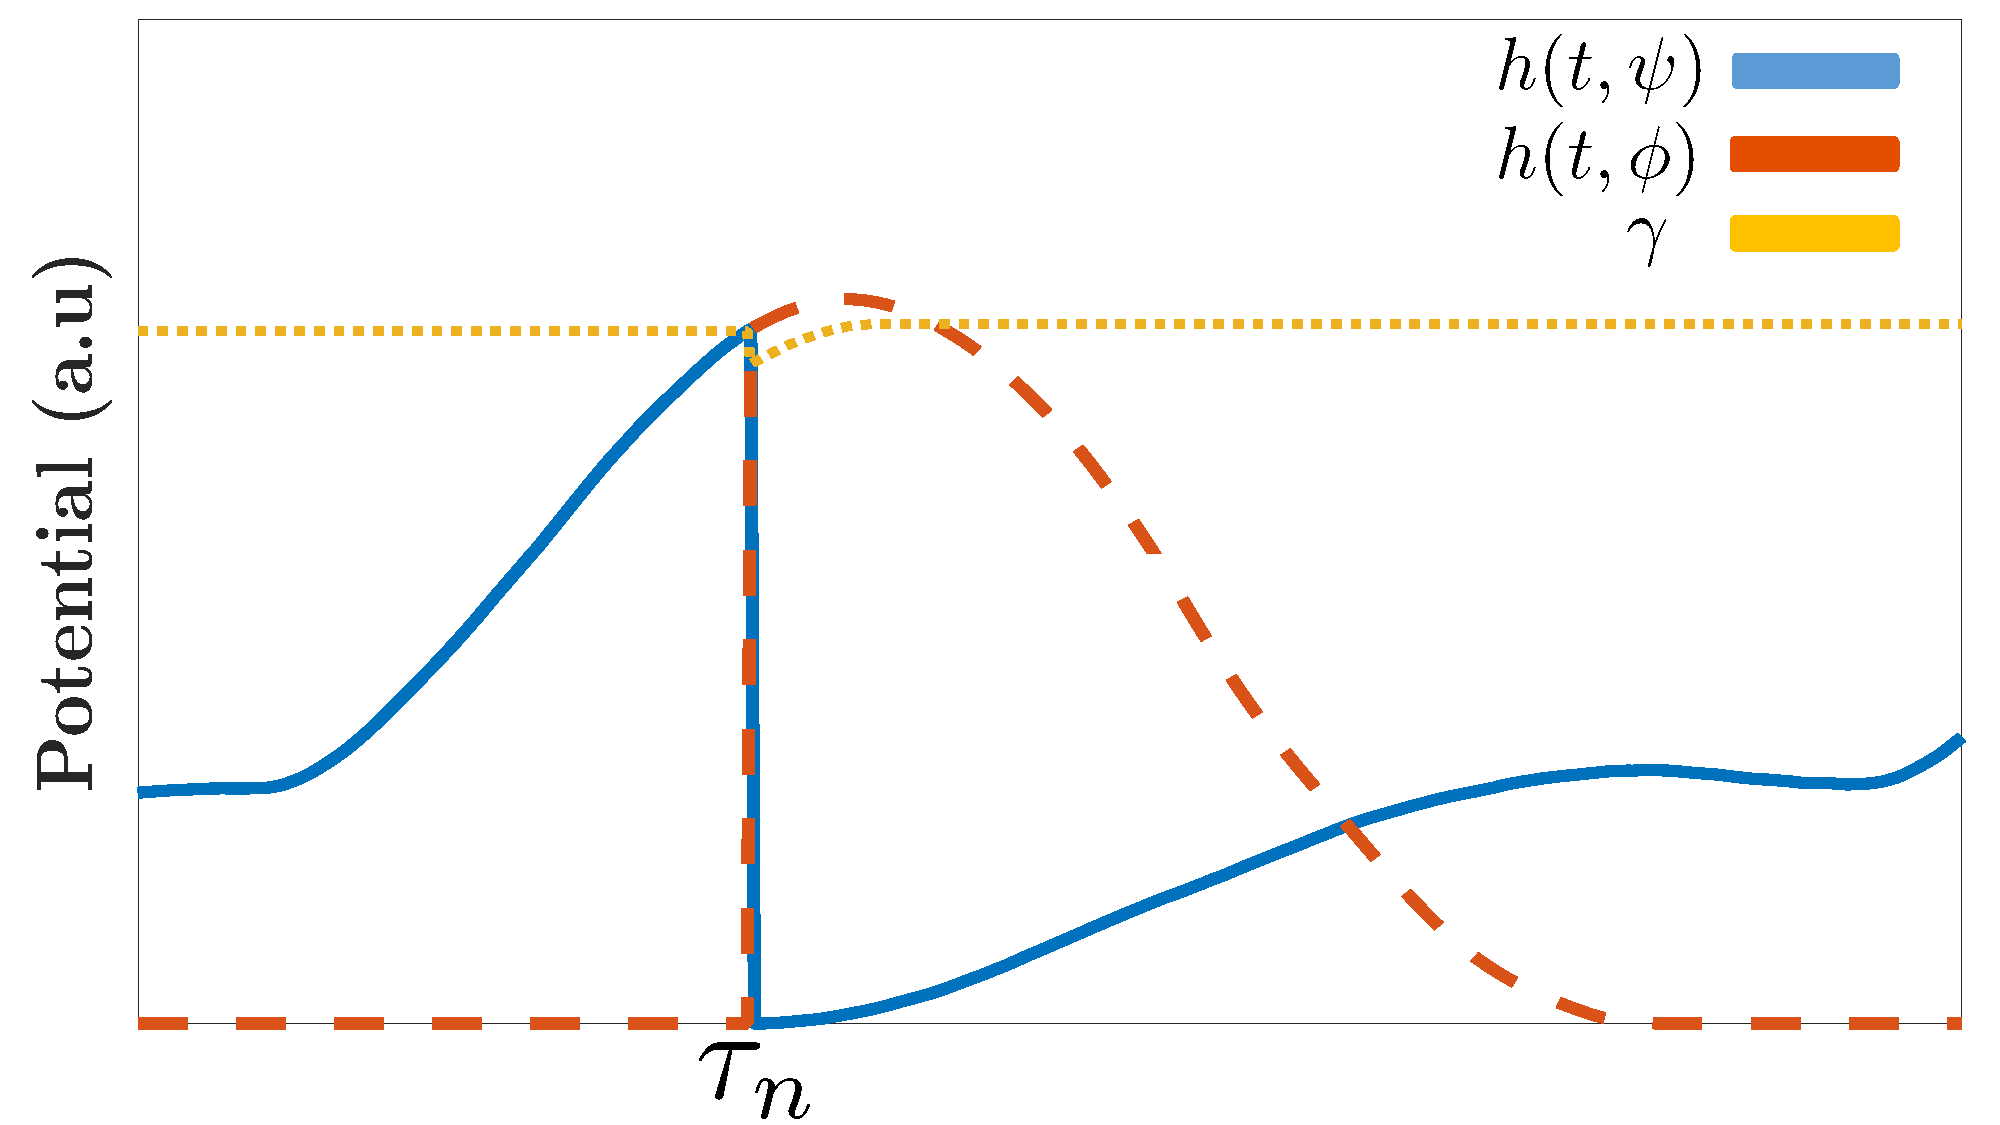
\includegraphics[width=0.5\textwidth,height=3.5cm]{Fig4}
\caption{\textbf{Contribution of Potential to Threshold}}
\label{fig:4}
\end{figure}          
%************************************************
%% 			  	 Learning Rules
% ***********************************************
\section*{Learning Rules} 
In the described neural architecture, there are two sets of parameters that must be learned, the vectors $\boldsymbol{\alpha}$ and $\boldsymbol{\beta}$ to approximate the delay function for each input given $\vec{T_\xi}$ and the threshold $\gamma$ of the neuron.
% ***********************************************
%%				Delay Function Updating 
% ***********************************************
\subsection*{Updating the Delay Function}
$\boldsymbol\alpha$ and $\boldsymbol\beta$ are initialized to $[2],[2]$ for all inputs. The rate of learning is adjustable based on a hyperparameter $\eta$ which determines the rate of change in the skew of an input activation time brought about by redistributing values in $\boldsymbol\alpha$ and $\boldsymbol\beta$. 

\paragraph{Weight Redistribution.}  Redistribution of $\alpha$ and $\beta$ values amongst a mixture of betas representing some input feature $f$ is important for winnowing out those component delay functions that do not significantly contribute to the neuron's potential while increasing the amplitude of the components with the largest peaks. Thus unused beta functions decay to 0, leaving only the input-specific components in the mixture. Weight redistribution is accomplished with two functions, \texttt{Subtract} and \texttt{Add Weights}. For each input, a variable $w$ is defined to represent the total sum of $\alpha$ and $\beta$ that must be redistributed amongst the mixtures composing that input.  A factor of $\eta$ is taken from all $\alpha$, $\beta$ pairs as shown in \texttt{Subtract Weight} (Algorithm \ref{alg:sub}).  The subtracted value $w$ is then added only to those pairs that contribute the most to $h(x)$, incrementing them in proportion to their total contribution (Algorithm \ref{alg:add}). The $\alpha$ and $\beta$ pairs that contribute most to the neuron's potential are identified by ordering all pairs from greatest to least using a function \texttt{ORDERED}. The contingency of additional inputs being encountered is addressed by function, \texttt{INCREASE}, in the add weights function.  This function evaluates whether a given input is activated more times than the number of $\alpha, \beta$ pairs for that input and if so adds additional pairs as required. 
\begin{algorithm}
\caption{Weight Subtraction}\label{alg:sub}
\begin{algorithmic}[1]
\Procedure{Subtract Weight}{}
\State $w\gets 0 $
\For{$s \in S$}
\For{$\alpha_j,\beta_j,\in \boldsymbol{\alpha_{s_i}}, \boldsymbol{\beta_{s_i}}$}
\State $w \gets w + \eta \alpha_j + \eta \beta_j$
\State $\alpha_j\gets \alpha_j - \eta \alpha_j$
\State $\beta_j\gets \beta_j - \eta \beta_j$
\EndFor
\EndFor
\State $w \gets w/|\phi|$
\State \Return $w$
\EndProcedure
\label{PC:SubW}
\end{algorithmic}
\end{algorithm}
\begin{algorithm}
\caption{Weight Addition}\label{alg:add}
\begin{algorithmic}[1]
\Procedure{Add Weight}{w}
\For{$s \in \{s \ | \ \tau_s \ \in \phi \} $}
\If{$| \ \tau_{s_i} \ | > |\vec{A_{s_i}}|$} \Comment{\# of activations $>$ than \# of distributions}
\State INCREASE($\boldsymbol{ \ \alpha_{s_i}}, \ |\ \tau_{s_i}\ | \ $) 
\State \uppercase{Increase}($\boldsymbol{\ \beta_{s_i}}, \ |\ \tau_{s_i}\ | \ $)
\EndIf
\State $count \gets 0$
\While{$count < \ |\  \tau_{s_i} \ | \ $}
\State $\alpha, \ \beta \gets $ORDERED($\boldsymbol{\ \alpha_{s_i}},\boldsymbol{\ \beta_{s_i}})[count]$
\State $ratio_\alpha \gets \alpha/(\alpha + \beta)$
\State $ratio_\beta \gets \beta/(\alpha + \beta)$
\State $\alpha \gets \alpha + w\ *$ \ ratio$_\alpha$
\State $\beta \gets \beta + w\ *$ \ ratio$_\beta$
\State $count \gets count + 1$
\EndWhile
\EndFor
\EndProcedure
\end{algorithmic}
\end{algorithm}
\paragraph{Skewing the Beta to Represent Structure in Time.} The skew in time of each component distribution is evaluated after the $\alpha, \beta$ weights have been redistributed towards the most contributing functions.  The process for skewing the beta functions comprising the mixture for each input is outlined in Algorithm \ref{alg:skew}.  Only the most contributing $\alpha, \beta$ pairs are skewed.  The skew is computed as the difference between the scaled firing time $z$ and the peak time of a given $\alpha, \beta$ pair.  A given component distribution is moved to the right/left if it occurs before/after firing time, $\tau_n$, resulting in entrainment of $\tau_n$ to occur at the end of pattern $\xi$.
\begin{algorithm}
\caption{Adjusting Skew of Delay}\label{alg:skew}
\begin{algorithmic}[1]
\Procedure{Skew}{}
\For{$s\in \{ s \ | \ \tau_s \in \phi \}$}
\State $counter\gets 0$
\While{$counter<|\{\tau_{s_i} \in \phi\}|$}
\State $\alpha, \ \beta = ORDERED (\boldsymbol{\alpha_{s_i}},\boldsymbol{\beta_{s_i}})[count]$
\State skew$=x-((\alpha-1)/(\alpha+\beta-2))$
\If{skew$<0$}\Comment{Peak of the distribution is to the right of $\tau_n$}
\State redist$\gets \alpha \eta * -$skew \Comment{Move peak to the left}
\State $\alpha \gets \alpha - redist$
\State $\alpha \gets \beta + redist$
\Else\Comment{Peak of the distribution is to the left of $\tau_n$}
\State $redist\gets \eta\beta*skew$ \Comment{Move peak to the right}
\State $\beta \gets \beta - redist$
\State $\alpha \gets \alpha + redist$
\EndIf
\EndWhile
\EndFor
\EndProcedure
\label{PC:Skew}
\end{algorithmic}
\end{algorithm}
% ***********************************************
%% 			  	  Thresholding  
% ***********************************************
\subsection*{Adaptive Thresholding} Recognition of a pattern $\xi$ embedded in a noisy time series occurs when $n$ exceeds a threshold $y$ and emits a spike.  The value of $\gamma$ must be set high enough to filter out noisy inputs but not too high so as to prevent $n$ from ever firing.  An adaptive threshold dependent on the total potential before and after firing is detailed in Algorithm \ref{alg:thresh}.  The threshold is incremented as a function of the total potential windowed around $\tau_n$ and multiplied by learning rate $\eta$.

\begin{algorithm}
\caption{Adaptive Threshold}\label{alg:thresh}
\begin{algorithmic}[1]
\Procedure{Update Threshold}{}
\If{$\eta * (h(t,\phi)+h(t,\psi))>\gamma$}
\State $\gamma \gets \eta * (h(t,\phi) + h(t,\psi))$
\EndIf
\If{$h(t,\phi)>\gamma$}
\State $\gamma \gets \eta * h(t,\phi)$
\EndIf
\EndProcedure
\end{algorithmic}
\end{algorithm}

% ***********************************************
%% 			  	 Simple Patterns 
% ***********************************************
\section*{Simple-Patterns}
Here we present preliminary results using the proposed learning algorithm on simple patterns.  Sounds composed of simple frequency sweeps in time with 200ms duration were generated and Fourier transformed to generate our $g(\vec{f}, \vec{t})$ which is a time-frequency spectrogram where  $\vec{f}$ is defined over the set of frequencies that sum linearly to reconstruct the original time-domain signal.  The algorithm was initialized with $\eta=0.1$ for both the threshold update and weight redistribution rule with 10 distributions composing the initial beta mixture.  The window was set to 1.5x the length of the pattern.  The network was trained and tested on left and right chevron shaped frequency sweeps in time both with and without 1:1 signal to noise ratio. Training on clean images resulted in 100\% classification accuracy after only 15 presentations.  The network also exhibited perfect performance noisy images resulted in 100\% classification accuracy but only after $50$ presentations (Figure \ref{fig:simplesims}).
\begin{figure}
\centering
\subfloat{
\subfloat[Clean Right Chevron]{
  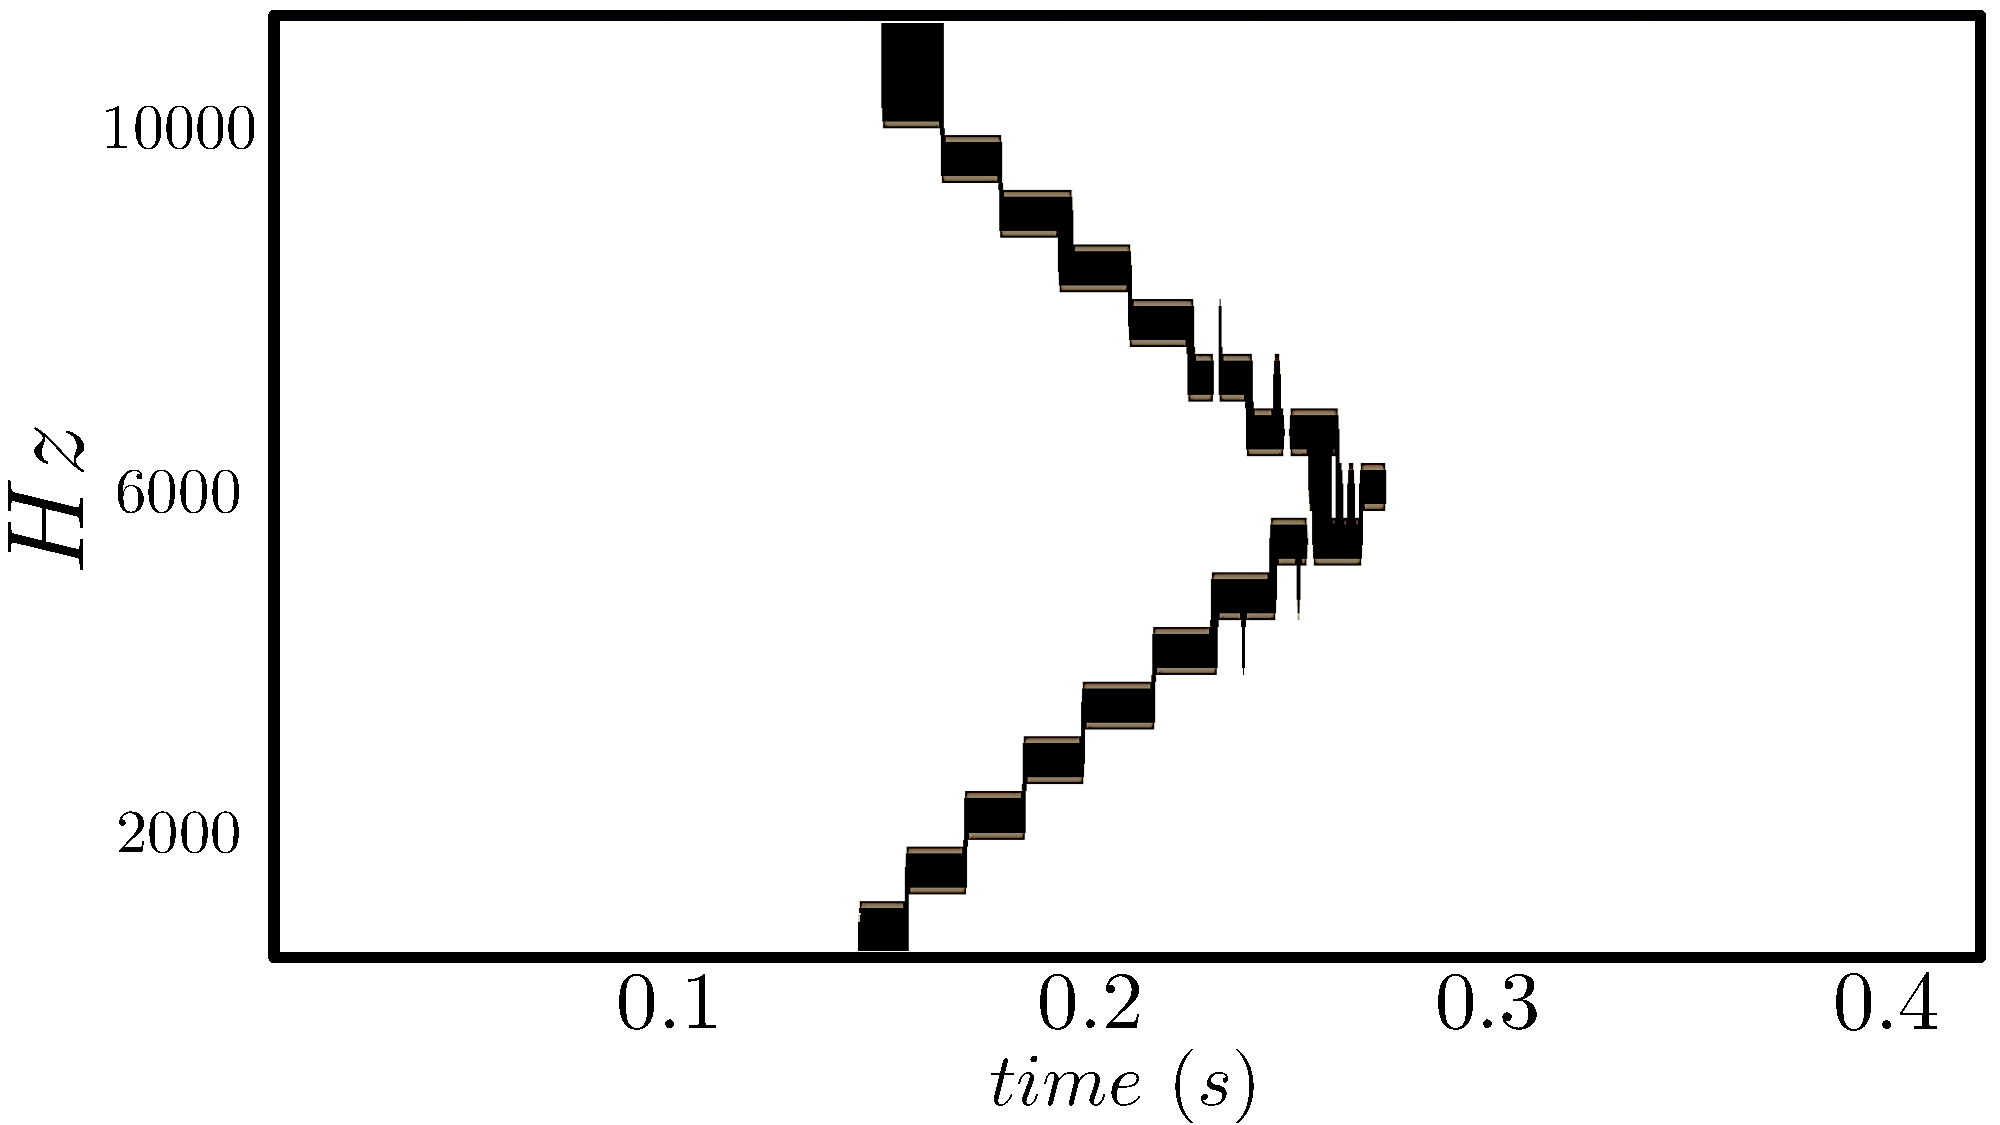
\includegraphics[width=0.25\textwidth]{Fig5A}
  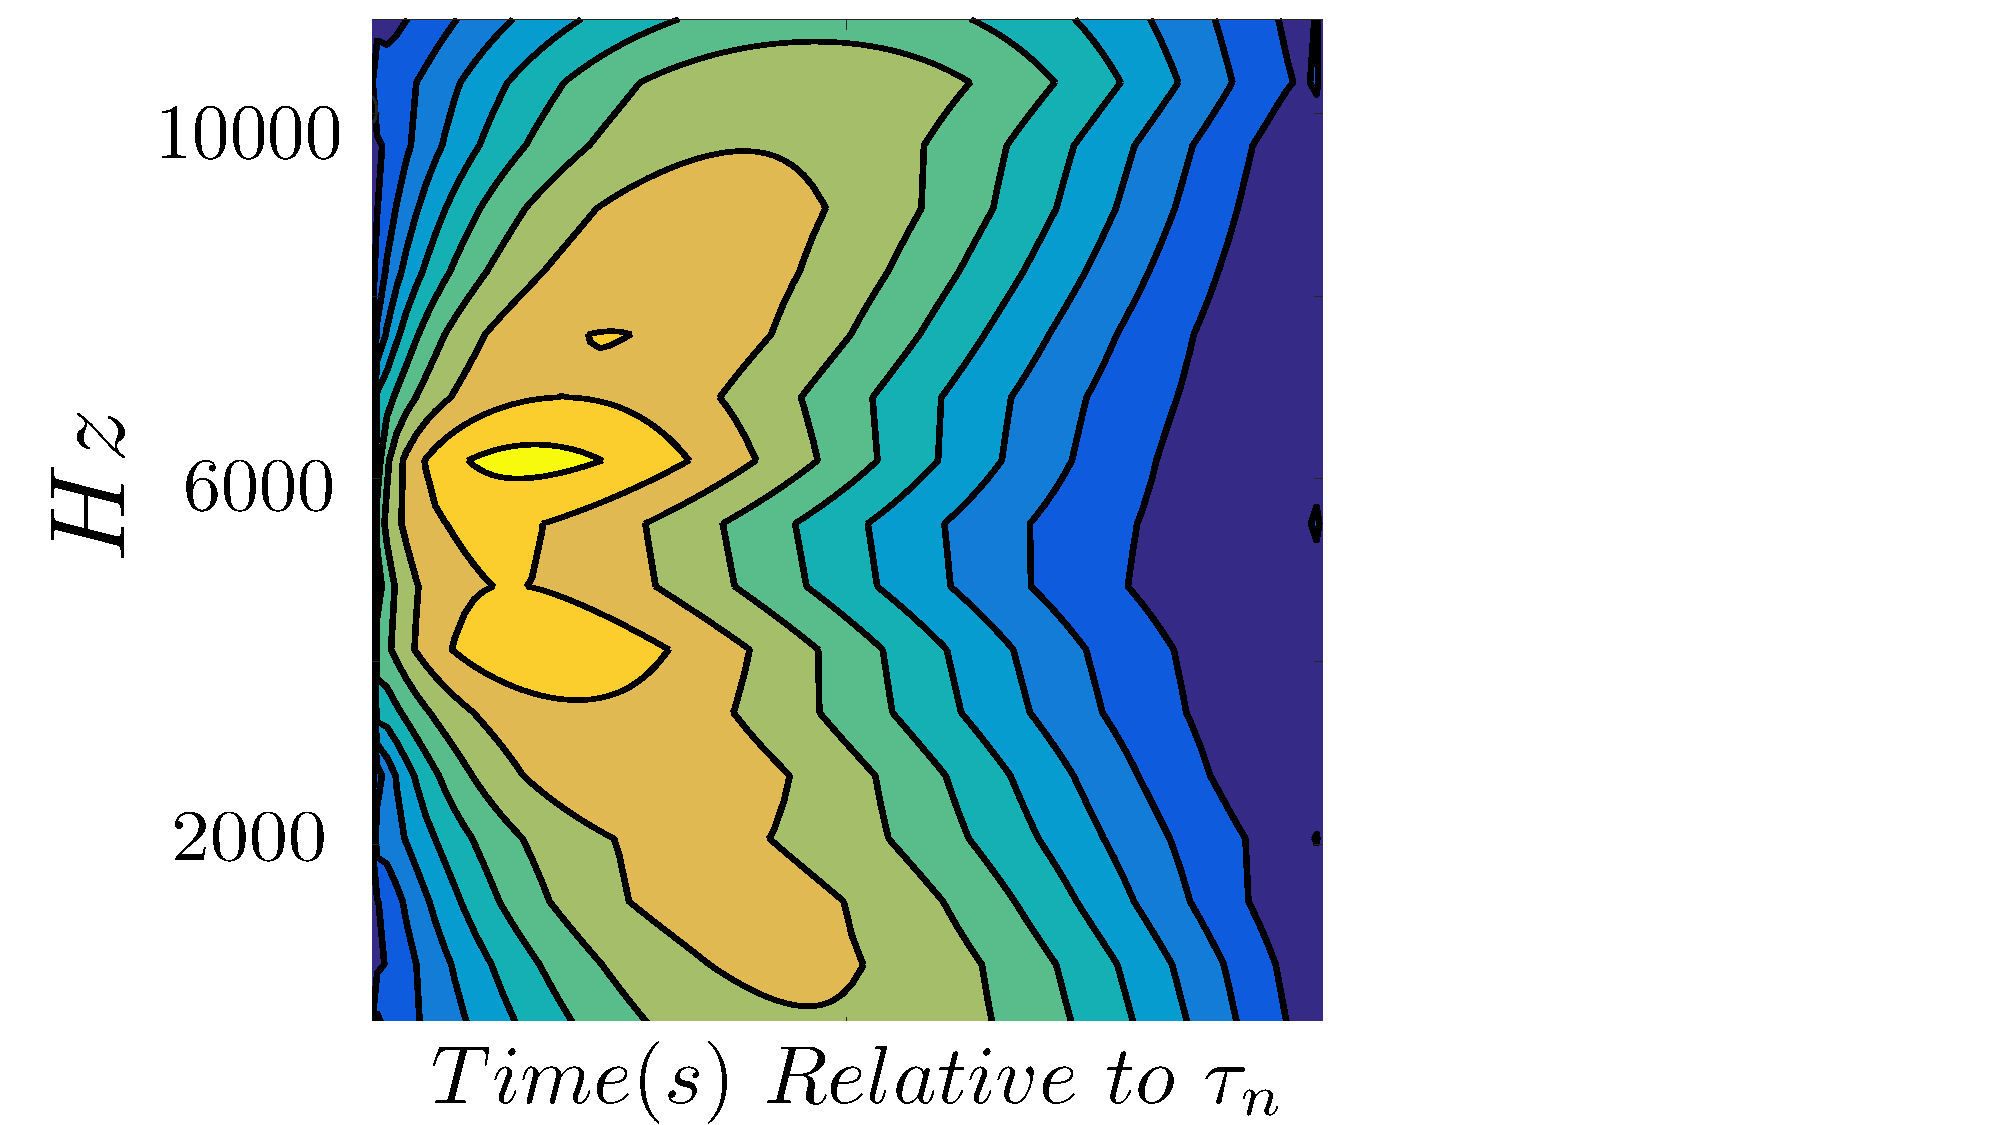
\includegraphics[width=0.25\textwidth]{Fig5B}
}
\hspace{0mm}
\subfloat[Clean Left Chevron]{
  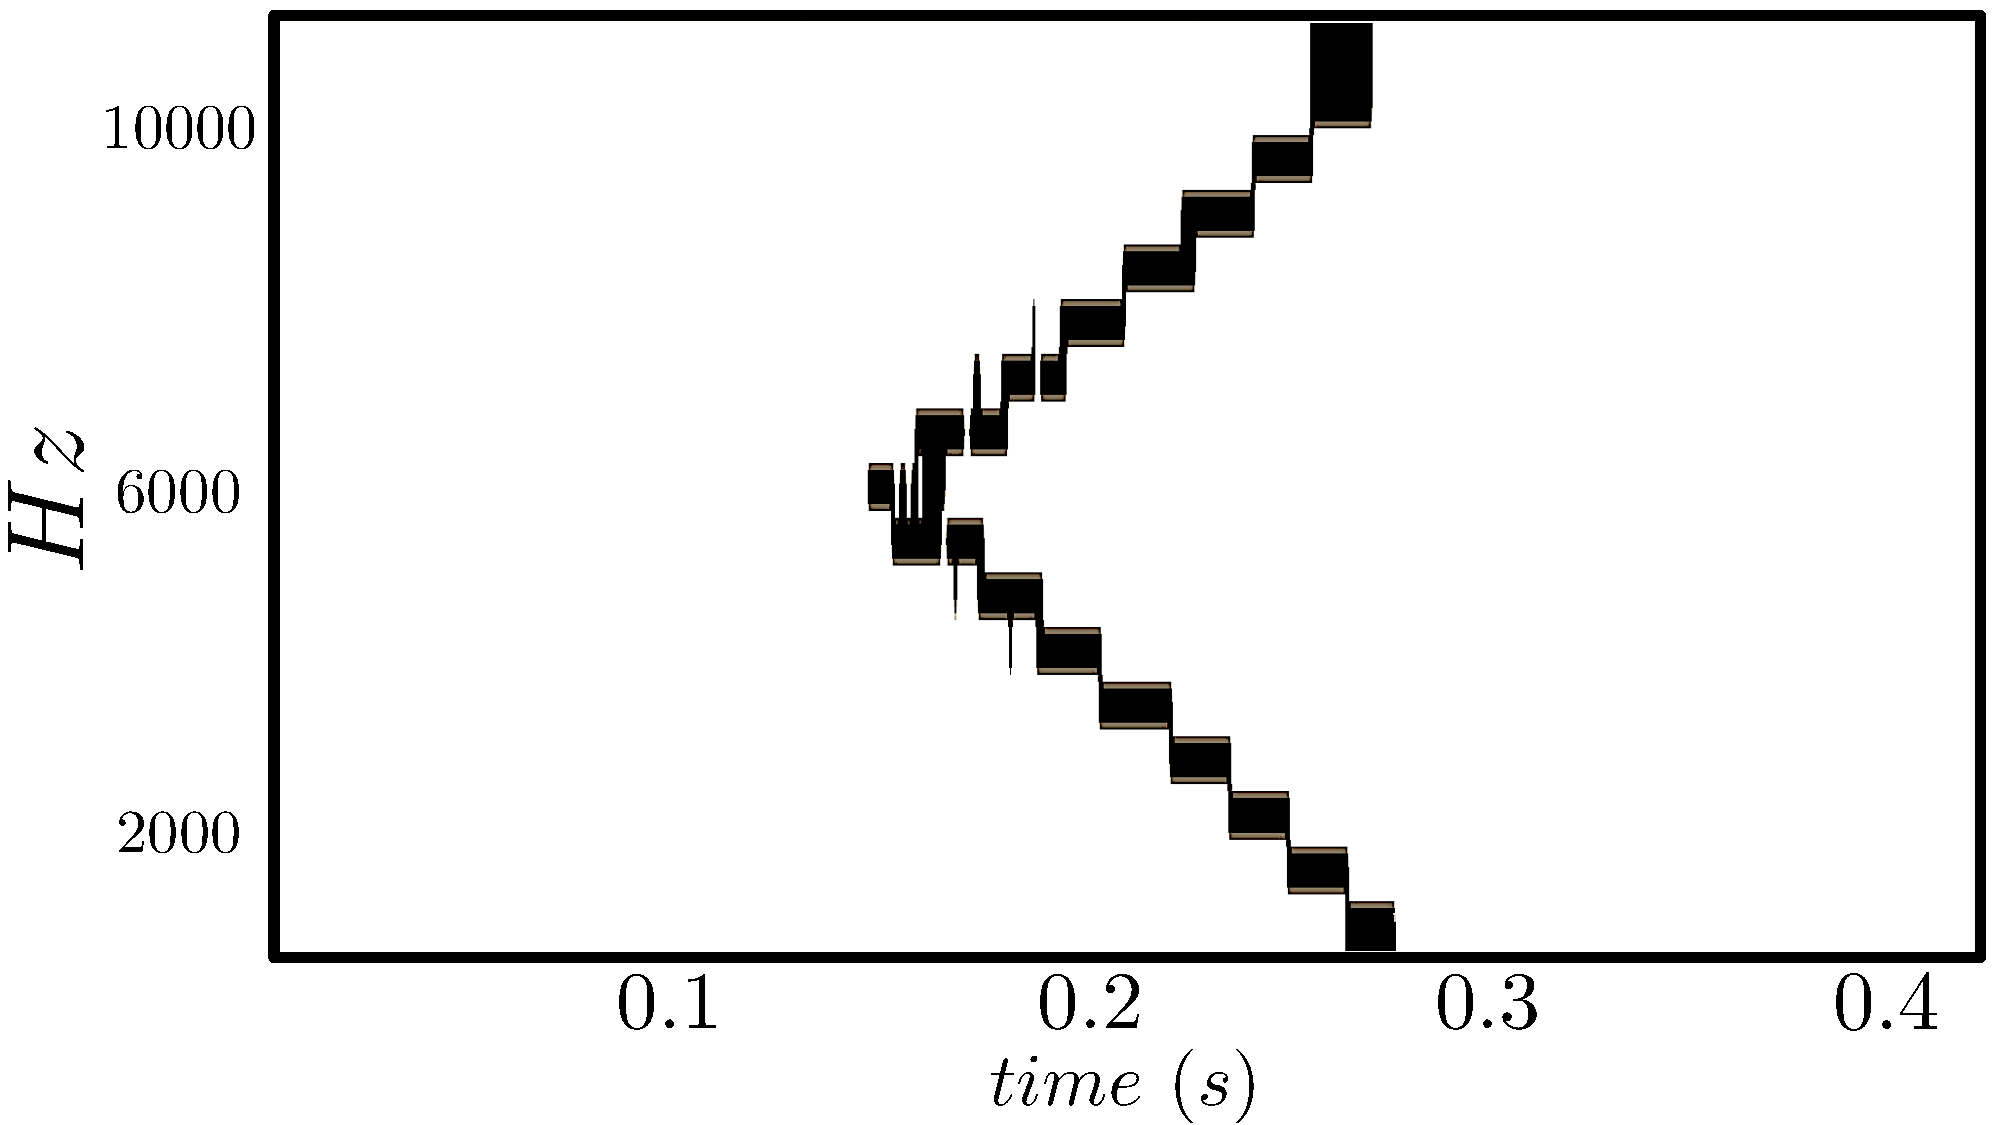
\includegraphics[width=0.25\textwidth]{Fig5C}
  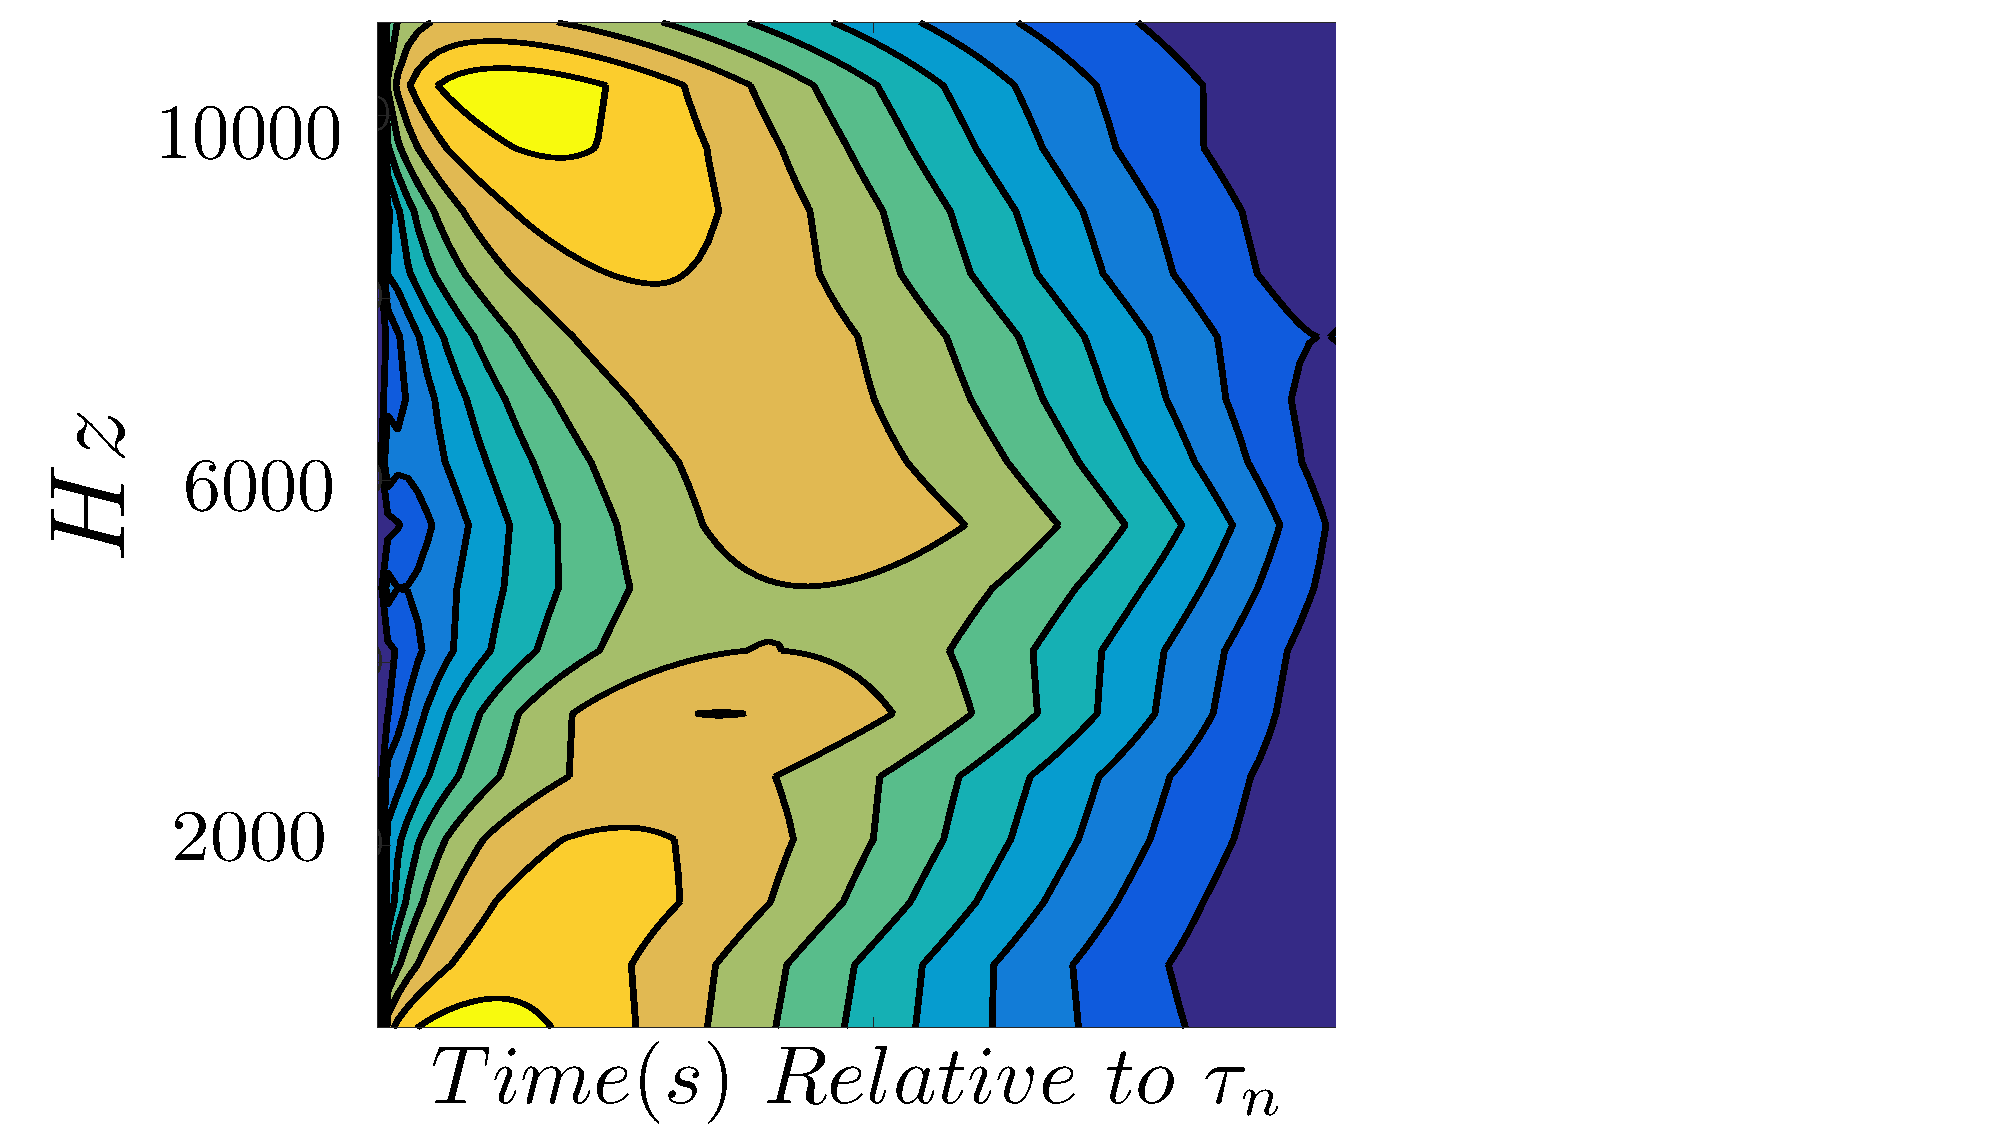
\includegraphics[width=0.25\textwidth]{Fig5D}
}}
\ 
\subfloat{
\hspace{0mm}
\subfloat[Noisy Right Chevron]{
  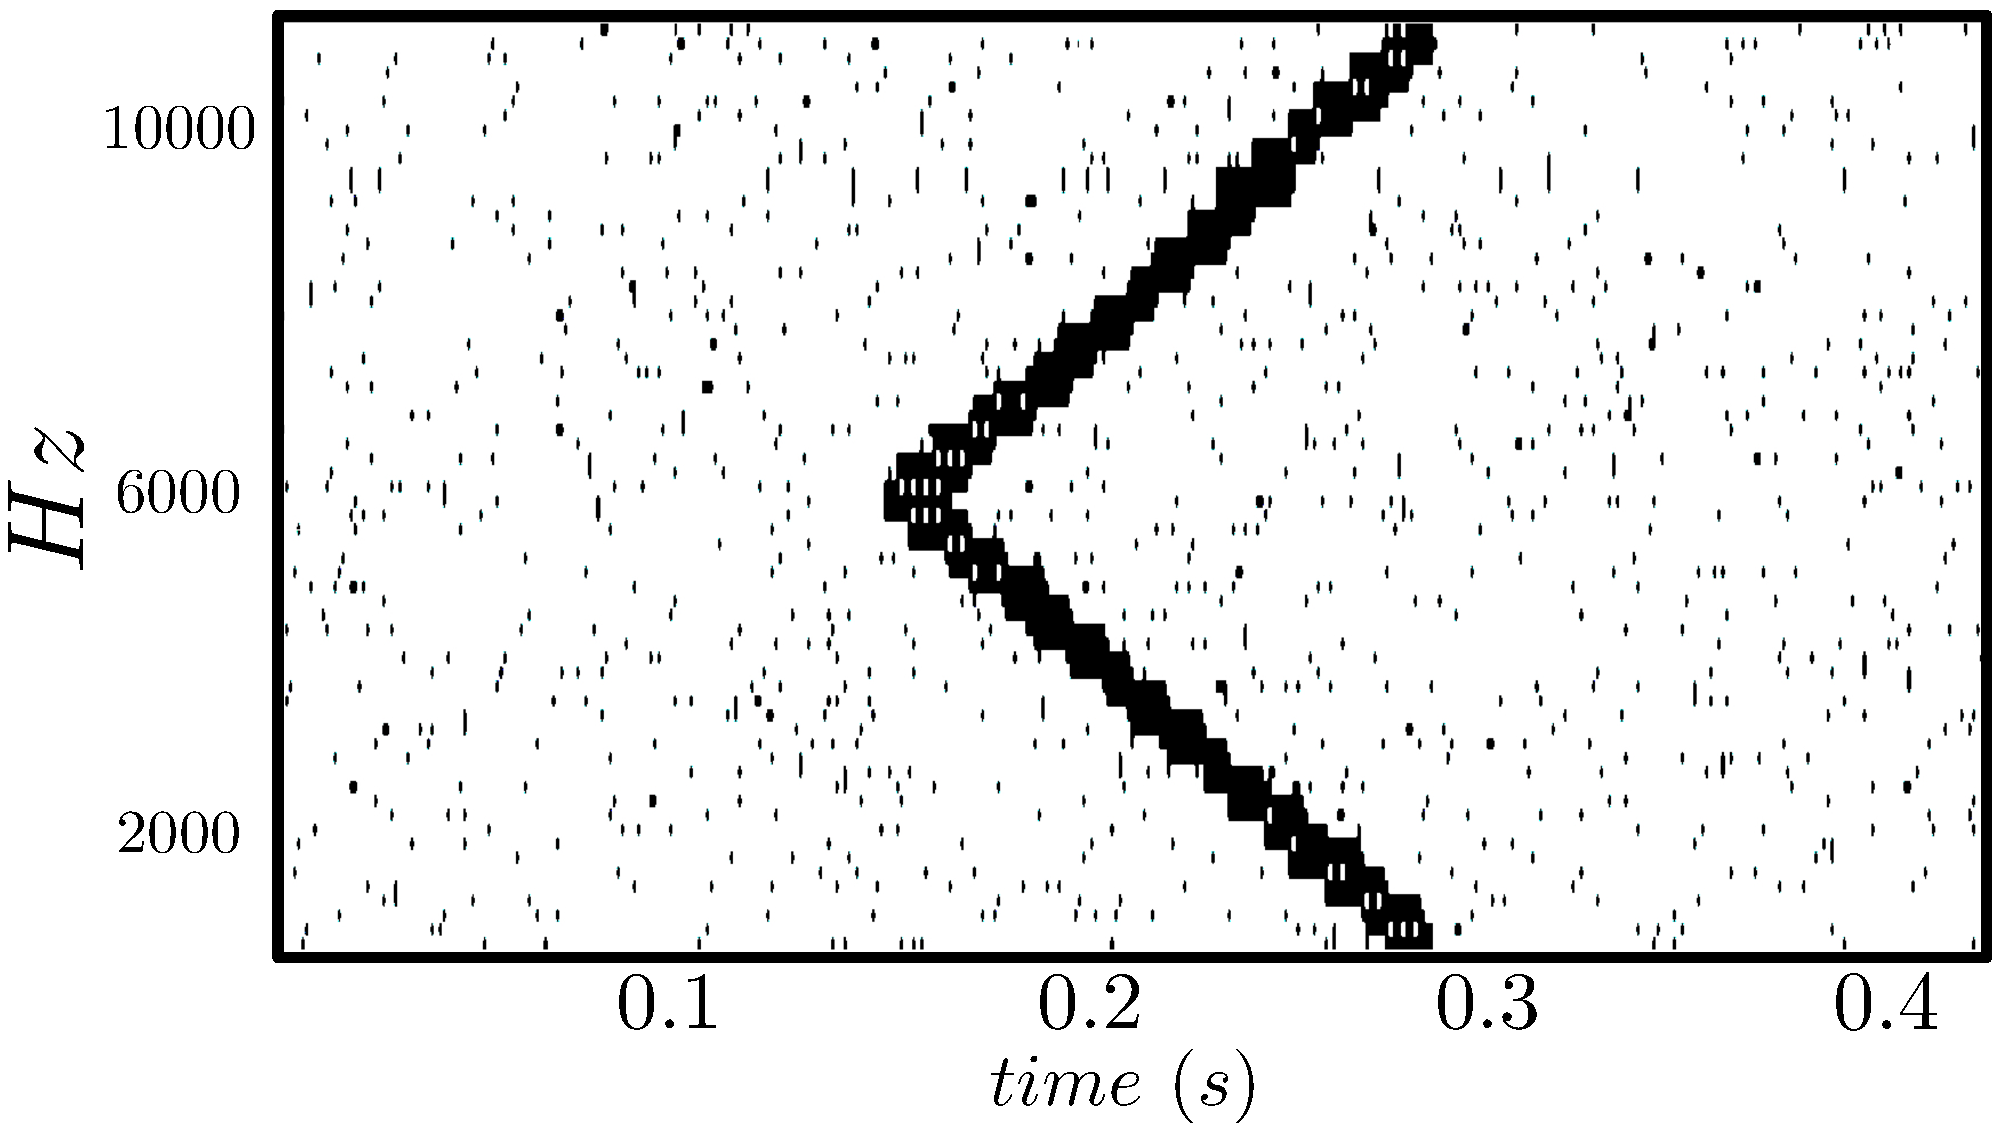
\includegraphics[width=0.25\textwidth]{Fig5E}
  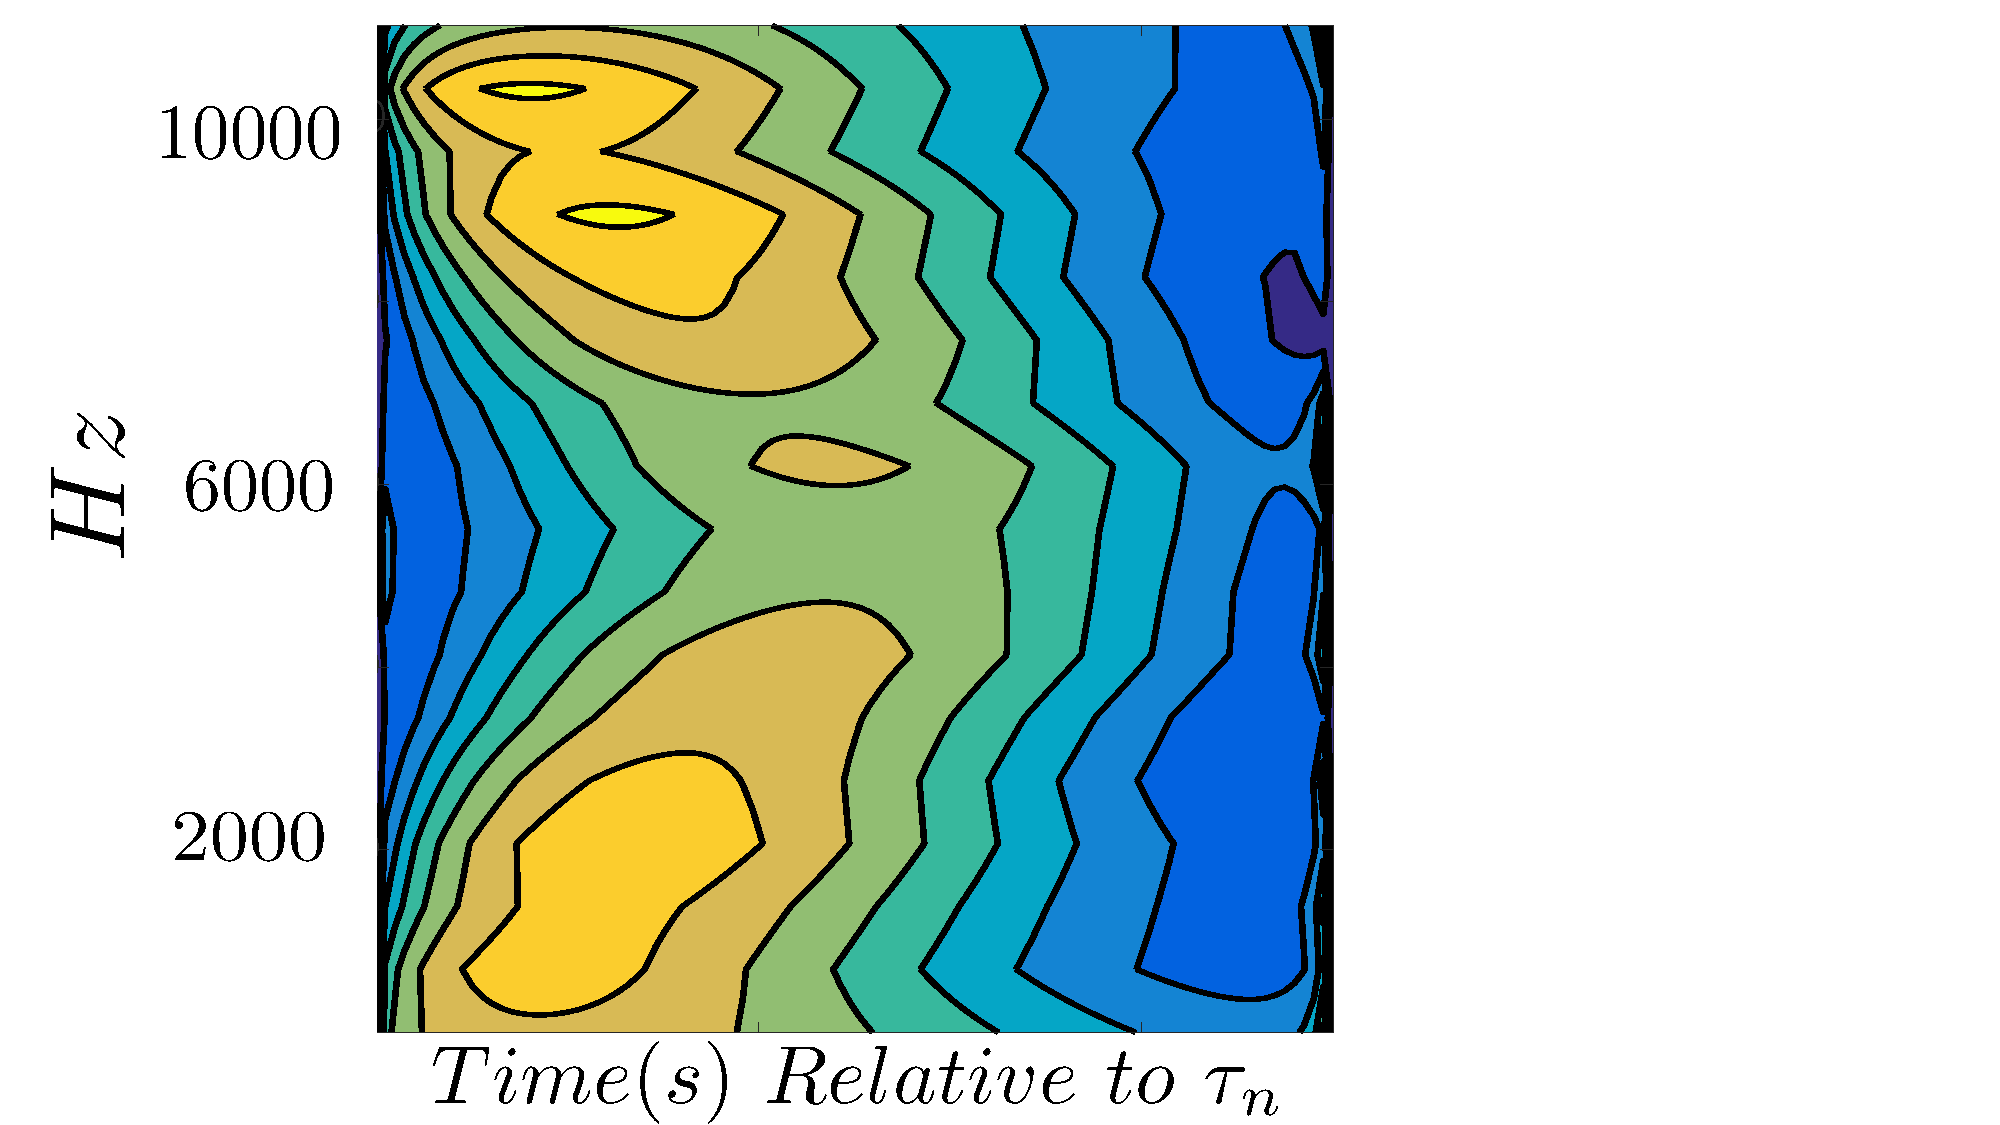
\includegraphics[width=0.25\textwidth]{Fig5F}
}
\hspace{0mm}
\subfloat[Noisy Left Chevron]{ 
  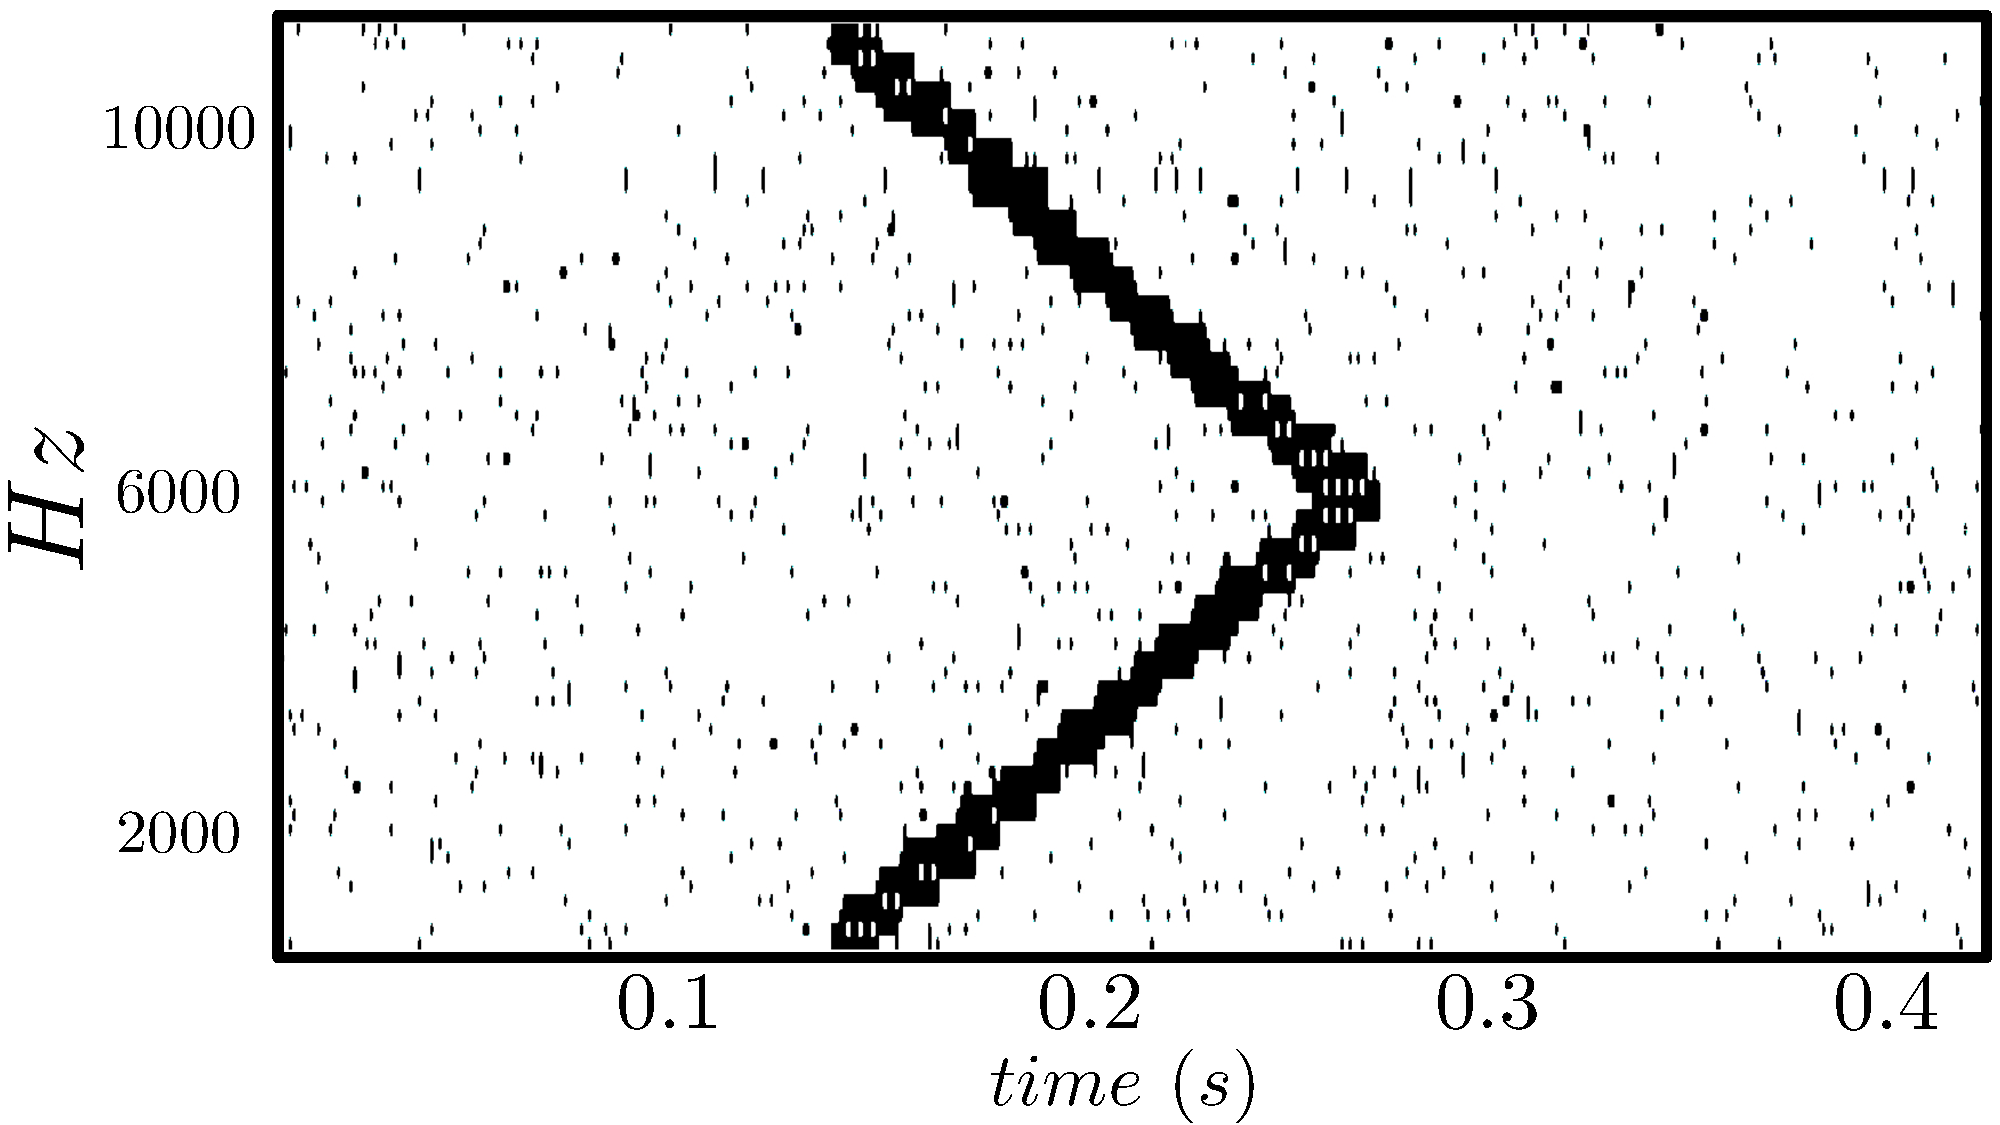
\includegraphics[width=0.25\textwidth]{Fig5G}
  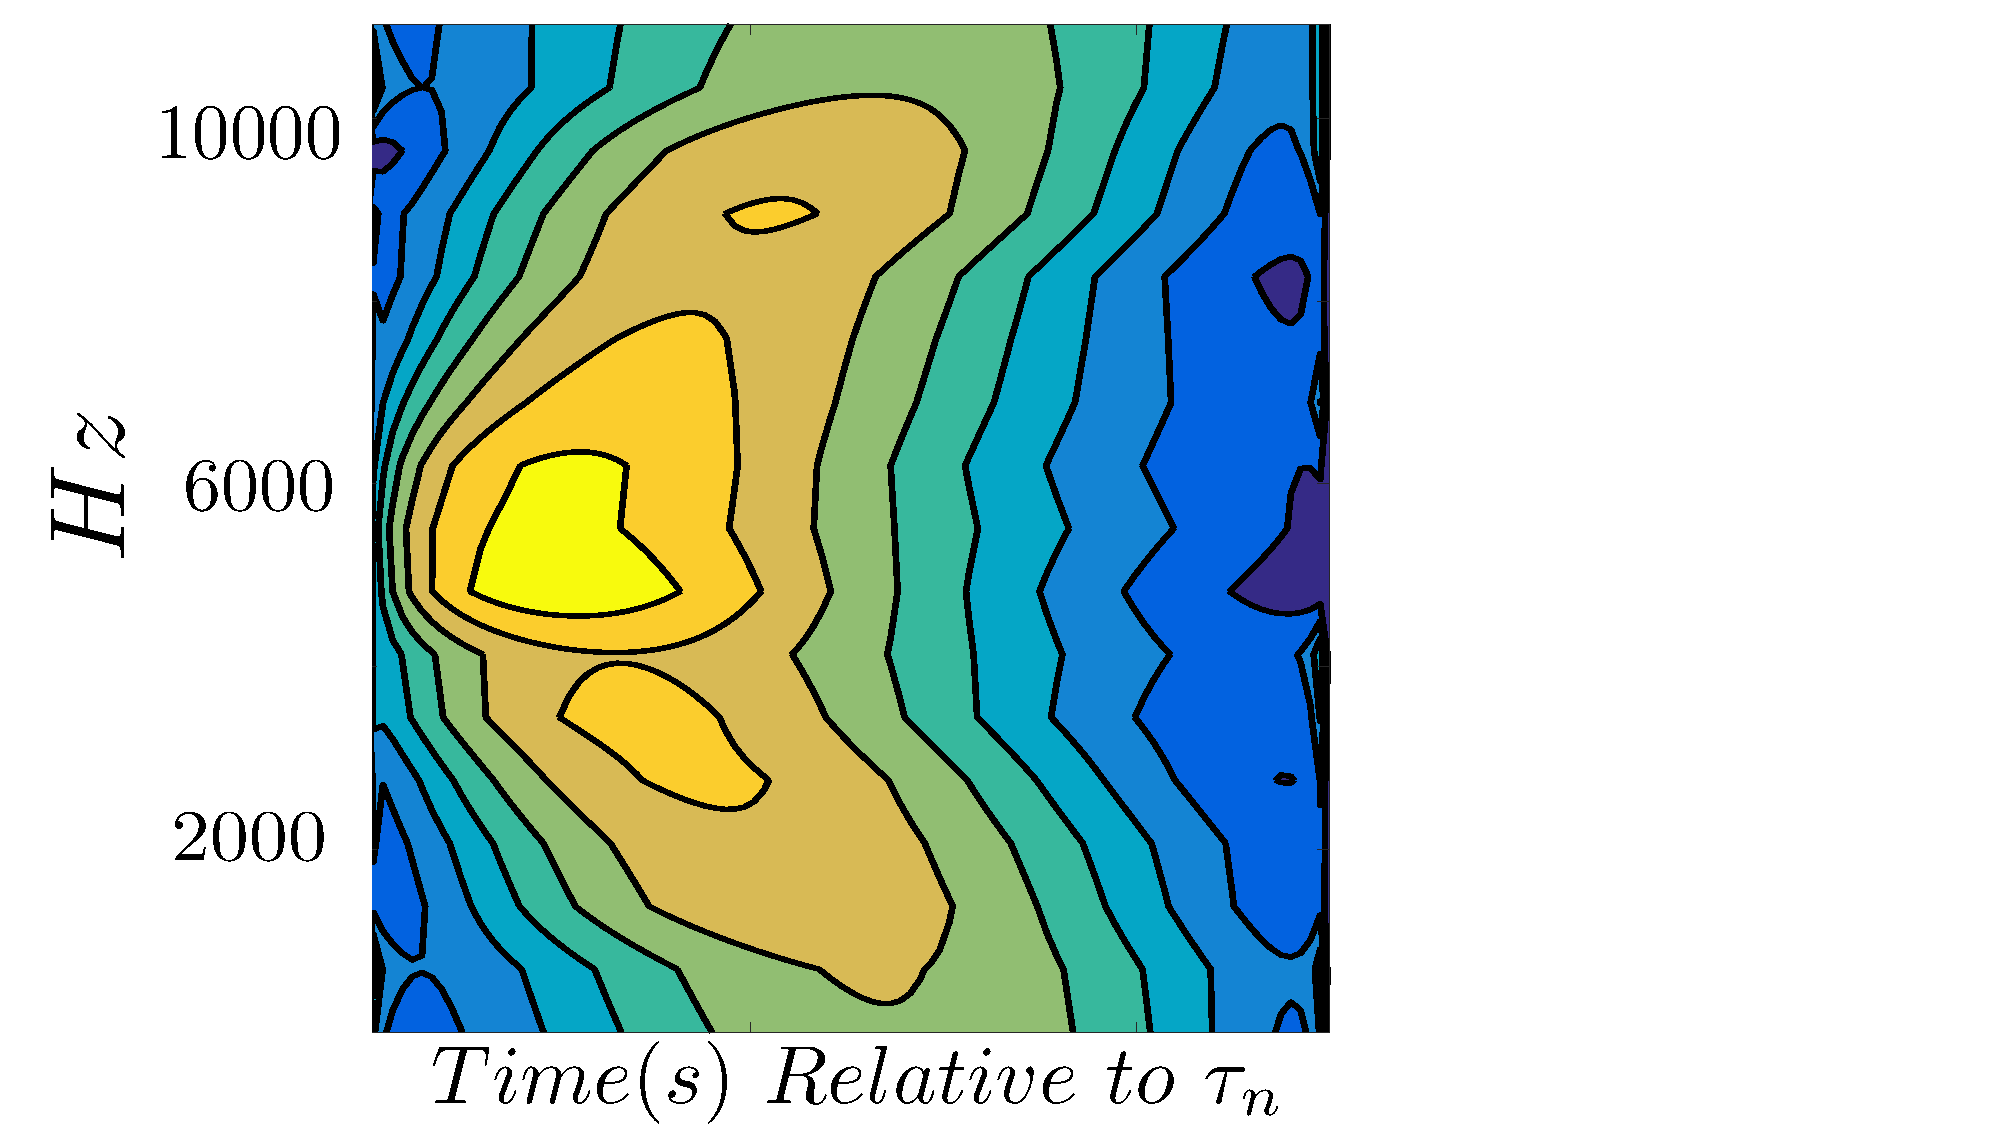
\includegraphics[width=0.25\textwidth]{Fig5H}
}}
\caption{\textbf{Model Network Performance.}  The model was trained on simple patterns with and without noise as shown in column 1.  The internal representation of the trained pattern is shown in column 2.  Note the internal representation is a mirror image of the input pattern since earlier inputs must be delayed greater features at the end of the pattern.}
\label{fig:simplesims}
\end{figure}
            
% ***********************************************
%% 			  	    Discussion
% ***********************************************
\section*{Discussion}
Here we propose a new model for unsupervised recognition of patterns nested within a noisy time series signal.  The model was able to learn different simple images embedded in noise with 100\% classification rate after only 50 training presentations.  The internal representation of the time delays in the form of the beta mixture was sharpened with training to reflect the arrival times of each of the feature inputs relative to neuron firing time.  The internal representation sharpens with increased training presentations and greater number of initial mixture components. Our results demonstrate the choice of a beta distribution for representing time delays of an input with adaptive thresholding is a promising method for development of unsupervised learning temporal pattern algorithms.  Future work is required to evaluate the performance of this algorithm on various temporal pattern structures and with different hyper parameter settings. 
% ***********************************************
%% 			  	   References
% ***********************************************
\section*{References}
\small
[1] Hopfield, J.J (1995) Pattern Recognition Computation Using Action Potential Timing for Stimulus Representation. {\it Nature} {\bf 376}(6):33-36.

[2] Hopfield, J.J (1996) Transforming Neural Computations and Representing Time. {\it Proc. Natl. Acad. Sci} {\bf 93}:15440-15444

[3] Izhikevich, E.M (2005) Polychronization: Computation with Spikes. {\it Neural Computation} {\bf 18}:245-282.

[3] Rekabdar, B., Nicolescu, M., Kelley R., \& Nicolescu, M. (2015) An Unsupervised Approach to Learning and Early Detection of Spatio-Temporal Patterns Using Spiking Neural Networks. {\it Intell Robot Sys} {\bf 80}:83-97

[4] Paugam-Moisy, H., Martinez, R., \& Bengio, S. (2006) A Supervised Learning Approach Based on STDP And Polychronization in Spiking Neuron Networks. {\it Proc. Natl. Acad. Sci} {\bf84}:1896-1900

[5] Tank, D.W. \& Hopfield, J.J (1987) Neural Computation by Concentrating Information in Time. {\it Proc. Natl. Acad. Sci} {\bf84}:1896-1900

[6] Waibel, A., Hanazawa, T.,\ Hinton, G.,\ Shikano, K., \& Lang, K.L\ (1989) Phoneme Recognition Using Time-Delay Neural Networks. {\it IEEE Transactions on Acoustics, Speech \& Signal Processing} {\bf 37}(3):328-338.

[7] Vries, B. \& Principe, J.C (1992) The Gamma Model - A New Neural Model for Temporal Processing. {\it Neural Networks} {\bf5}:565-576

\end{document}
